\documentclass[twoside]{book}

% Packages required by doxygen
\usepackage{calc}
\usepackage{doxygen}
\usepackage{graphicx}
\usepackage[utf8]{inputenc}
\usepackage{makeidx}
\usepackage{multicol}
\usepackage{multirow}
\usepackage{textcomp}
\usepackage[table]{xcolor}

% Font selection
\usepackage[T1]{fontenc}
\usepackage{mathptmx}
\usepackage[scaled=.90]{helvet}
\usepackage{courier}
\usepackage{amssymb}
\usepackage{sectsty}
\renewcommand{\familydefault}{\sfdefault}
\allsectionsfont{%
  \fontseries{bc}\selectfont%
  \color{darkgray}%
}
\renewcommand{\DoxyLabelFont}{%
  \fontseries{bc}\selectfont%
  \color{darkgray}%
}

% Page & text layout
\usepackage{geometry}
\geometry{%
  a4paper,%
  top=2.5cm,%
  bottom=2.5cm,%
  left=2.5cm,%
  right=2.5cm%
}
\tolerance=750
\hfuzz=15pt
\hbadness=750
\setlength{\emergencystretch}{15pt}
\setlength{\parindent}{0cm}
\setlength{\parskip}{0.2cm}
\makeatletter
\renewcommand{\paragraph}{%
  \@startsection{paragraph}{4}{0ex}{-1.0ex}{1.0ex}{%
    \normalfont\normalsize\bfseries\SS@parafont%
  }%
}
\renewcommand{\subparagraph}{%
  \@startsection{subparagraph}{5}{0ex}{-1.0ex}{1.0ex}{%
    \normalfont\normalsize\bfseries\SS@subparafont%
  }%
}
\makeatother

% Headers & footers
\usepackage{fancyhdr}
\pagestyle{fancyplain}
\fancyhead[LE]{\fancyplain{}{\bfseries\thepage}}
\fancyhead[CE]{\fancyplain{}{}}
\fancyhead[RE]{\fancyplain{}{\bfseries\leftmark}}
\fancyhead[LO]{\fancyplain{}{\bfseries\rightmark}}
\fancyhead[CO]{\fancyplain{}{}}
\fancyhead[RO]{\fancyplain{}{\bfseries\thepage}}
\fancyfoot[LE]{\fancyplain{}{}}
\fancyfoot[CE]{\fancyplain{}{}}
\fancyfoot[RE]{\fancyplain{}{\bfseries\scriptsize Generated on Fri Jul 1 2016 12\-:32\-:42 for Yarp\-Bottle\-Generator by Doxygen }}
\fancyfoot[LO]{\fancyplain{}{\bfseries\scriptsize Generated on Fri Jul 1 2016 12\-:32\-:42 for Yarp\-Bottle\-Generator by Doxygen }}
\fancyfoot[CO]{\fancyplain{}{}}
\fancyfoot[RO]{\fancyplain{}{}}
\renewcommand{\footrulewidth}{0.4pt}
\renewcommand{\chaptermark}[1]{%
  \markboth{#1}{}%
}
\renewcommand{\sectionmark}[1]{%
  \markright{\thesection\ #1}%
}

% Indices & bibliography
\usepackage{natbib}
\usepackage[titles]{tocloft}
\setcounter{tocdepth}{3}
\setcounter{secnumdepth}{5}
\makeindex

% Hyperlinks (required, but should be loaded last)
\usepackage{ifpdf}
\ifpdf
  \usepackage[pdftex,pagebackref=true]{hyperref}
\else
  \usepackage[ps2pdf,pagebackref=true]{hyperref}
\fi
\hypersetup{%
  colorlinks=true,%
  linkcolor=blue,%
  citecolor=blue,%
  unicode%
}

% Custom commands
\newcommand{\clearemptydoublepage}{%
  \newpage{\pagestyle{empty}\cleardoublepage}%
}


%===== C O N T E N T S =====

\begin{document}

% Titlepage & ToC
\hypersetup{pageanchor=false}
\pagenumbering{roman}
\begin{titlepage}
\vspace*{7cm}
\begin{center}%
{\Large Yarp\-Bottle\-Generator }\\
\vspace*{1cm}
{\large Generated by Doxygen 1.8.6}\\
\vspace*{0.5cm}
{\small Fri Jul 1 2016 12:32:42}\\
\end{center}
\end{titlepage}
\clearemptydoublepage
\tableofcontents
\clearemptydoublepage
\pagenumbering{arabic}
\hypersetup{pageanchor=true}

%--- Begin generated contents ---
\chapter{Main Page}
\label{index}\hypertarget{index}{}\hypertarget{index_intro_sec}{}\section{Brief description}\label{index_intro_sec}
This project generates C++ code from a configuration text file that describes the set of inputs (i.\-e. ports/topics and their types), data conversions that may be applied to the inputs, and a detailed specification of the output (i.\-e. list of types, hierarchically defined). The yarp bottle generator parses a configuration file creates a C++ file. After compiling the C++ file and subsequent execution, the result acts as a bridge between Y\-A\-R\-P and R\-O\-S. The generated code reads data from several inputs (Y\-A\-R\-P ports or R\-O\-S topics), and constructs a Y\-A\-R\-P Bottle as output. Note that the yarp bottle generator has two modes of operation\-: (i) From R\-O\-S topics to a Y\-A\-R\-P port (R\-O\-S-\/\-Y\-A\-R\-P mode) and (ii) from Y\-A\-R\-P ports to a R\-O\-S topic (Y\-A\-R\-P-\/\-R\-O\-S mode). On one hand, reading from/sending to Y\-A\-R\-P ports is straightforward because our code generator is based on Y\-A\-R\-P bottles. On the other hand, reading from/sending to R\-O\-S topics needs an additional conversion, which is handled by the run-\/time Y\-A\-R\-P to R\-O\-S converter yarpidl\-\_\-rosmsg. 
\chapter{yarp-\/bottle-\/generator}
\label{md__home_plinio_Software_yarp-bottle-generator_README}
\hypertarget{md__home_plinio_Software_yarp-bottle-generator_README}{}
Although this repository is integrated within \href{https://github.com/vislab-tecnico-lisboa}{\tt Vis\-Lab}'s projects, it holds the result of my (\href{https://github.com/mikearagao}{\tt Miguel Aragão}) master thesis.

\subsection*{Brief description}

The main goal of the yarp-\/bottle-\/generator is for it to be able to generate code that gets data from several sources (Y\-A\-R\-P ports or R\-O\-S topics) and builds a bottle to be sent to some specific R\-O\-S topic or Y\-A\-R\-P port.

The final user will only have to customize a configuration file according to his needs.

For now there are 3 main structures that the user can customize\-: the multiplexers (i.\-e. hubs), the converters and the output builder (described in a R\-O\-S message style). Please read the documentation on \href{https://github.com/vislab-tecnico-lisboa/yarp-bottle-generator#configure-your-own-configuration-file}{\tt how to customize your own configuration file} in order to understand how they work and what you can achieve with them.

\subsection*{Dependencies}

The repository has two major dependencies\-:
\begin{DoxyItemize}
\item C\-Make -\/ needed to build the project
\item Boost -\/ the project uses several functionalities from the boost library
\end{DoxyItemize}

The code was written in C++ so any environment able to compile it (and compatible with the dependencies) should be fine.

\subsection*{Download}

Open a terminal\-: \begin{DoxyVerb}cd /path/to/destination/folder
git clone https://github.com/vislab-tecnico-lisboa/yarp-bottle-generator.git
\end{DoxyVerb}


\subsection*{Set the environment variable}

In order to run the generator you'll need to export the \$\-B\-O\-T\-T\-L\-E\-\_\-\-G\-E\-N\-E\-R\-A\-T\-O\-R\-\_\-\-D\-I\-R. Add the export to a script or execute it each time you want to run the generator\-: \begin{DoxyVerb}export BOTTLE_GENERATOR_DIR = /path/to/destination/folder/yarp-bottle-generator
\end{DoxyVerb}


\subsection*{Compile the generator}

Open a terminal\-: \begin{DoxyVerb}cd $BOTTLE_GENERATOR_DIR
mkdir build
cd build
cmake ..
make
\end{DoxyVerb}


Optionally you can copy the executable to your bin folder (and be able to run it from everywhere)\-: \begin{DoxyVerb}sudo make install
\end{DoxyVerb}


\subsection*{Generate a node with the default configuration file}

Open a terminal\-: \begin{DoxyVerb}yarpBottleGenerator
\end{DoxyVerb}


in order to see the command arguments\-: \begin{DoxyVerb}args:
[0]: configuration file name
[1]: generated code file name
\end{DoxyVerb}


In case you didn't run {\ttfamily sudo make install} you might need to run the last command from your build folder\-: \begin{DoxyVerb}cd $BOTTLE_GENERATOR_DIR/build
./yarpBottleGenerator <configuration file> <filename_generated_code.cpp>
\end{DoxyVerb}


The configuration file must be located in the app folder of the repository, and the generated code will be located in a folder inside the results folder of the repository. The filename of the generated code should have the .cpp extension.

\subsection*{Compile the generated node}

Open a terminal\-: \begin{DoxyVerb}cd $BOTTLE_GENERATOR_DIR/results/<filename_generated_code>
mkdir build
cd build
cmake ..
make
\end{DoxyVerb}


That's it! In case you didn't change the generated code yourself this should compile with no errors. Please open an issue in case you are having problems compiling unchanged generated code.

Feel free to edit the code to add some extra functionality at your own risk. Please open an issue if you think those changes should be automated to other users. I'll be available to help you with any doubts and problems.

\subsection*{Run the generated node}

Don't forget this is a Y\-A\-R\-P executable so you'll need to have a {\ttfamily yarpserver} running in order to run the code and if you are interacting with R\-O\-S, the runtime converter {\ttfamily yarpidl\-\_\-rosmsg} must be running as well.

Open a terminal\-: \begin{DoxyVerb}yarpserver
yarpidl_rosmsg
\end{DoxyVerb}


Execute your existing Y\-A\-R\-P modules and/or R\-O\-S nodes, and the code generated by yarp-\/bottle-\/generator.

\subsection*{Customize your own configuration file}

The interesting stuff starts now!

I recommend you to read the previous paragraphs to understand how to setup the envinronment and run the code in case you didn't do it already.

I'll split this documentation in 3 parts\-: general, multiplexers and message builder. In the current state of the development Y\-O\-U'L\-L H\-A\-V\-E T\-O C\-O\-N\-F\-I\-G\-U\-R\-E A\-L\-L T\-H\-E 4 P\-A\-R\-T\-S in order to correctly customize your own configuration file.

In the folder {\ttfamily \$\-B\-O\-T\-T\-L\-E\-\_\-\-G\-E\-N\-E\-R\-A\-T\-O\-R\-\_\-\-D\-I\-R/app}, create a text file that you have to edit in order to run the generator with your own configuration.

\subsubsection*{General}

\paragraph*{Sections}

This part has 1 section\-: {\ttfamily \mbox{[}general\mbox{]}}.

\subparagraph*{Section \mbox{[}general\mbox{]}}

It has 3 variables\-: {\ttfamily output\-\_\-name}, {\ttfamily to\-\_\-ros} and {\ttfamily num\-\_\-mux}.

{\ttfamily output\-\_\-name} \-: The name of the output topic/port. The bottle will be sent to this topic/port.

{\ttfamily to\-\_\-ros} \-: This variable expects true or false, true when the module is supposed to send a message to a R\-O\-S topic and false when the output is a Y\-A\-R\-P port.

{\ttfamily from\-\_\-ros\-\_\-topics} \-: This flag serves to decide if the input entities are ports or topics. Currently the supported data types are the ones translated by the run-\/time converter {\ttfamily yarpidl\-\_\-rosmsg}.

{\ttfamily num\-\_\-mux} \-: The number of multiplexers (i.\-e. Hubs) you want to create.

\paragraph*{Example}

\begin{DoxyVerb}[general]
output_name = /topic_name
to_ros = true
num_mux = 3
\end{DoxyVerb}


\subsubsection*{Multiplexers (i.\-e. Hubs)}

\paragraph*{Sections}

This part has 0 or more sections\-: {\ttfamily \mbox{[}mux1\mbox{]}...\mbox{[}muxn\mbox{]}}.

The generator expects an equal number of multiplexers and converters so the variables to configure the converter are in each multiplexer section (the last 2 variables are the ones that configure the converter).

\subparagraph*{Sections \mbox{[}mux1\mbox{]}...\mbox{[}muxn\mbox{]}}

They have 4 variables\-: {\ttfamily num\-\_\-ports}, {\ttfamily ports}, {\ttfamily function} and {\ttfamily verbose}.

{\ttfamily num\-\_\-ports} \-: The number of input ports/topics on the multiplexer.

{\ttfamily ports} \-: The name of all the input ports/topics. Each input name should be separated by a comma (in the end the number of commas should be equal to {\ttfamily num\-\_\-ports -\/ 1}). All white spaces will be excluded from the input names.

{\ttfamily function} \-: The name of one of the available functions (list of functions above). Each function expects specific arguments so be careful to specify a function compatible with the data contained on the multiplexer.

List of functions\-:


\begin{DoxyItemize}
\item {\ttfamily none} \-: This is a dummy function that has no effect on the multiplexer data. Use it when you want your converter to have no effect at all.
\item {\ttfamily none\-\_\-double} \-: Expects {\ttfamily double} values (or at least something that can be casted to {\ttfamily double}) so the multiplexer should only contain compatible values. Similar to the {\ttfamily none} function because it doesn't affect the multiplexer data. The main difference is that when the {\ttfamily verbose} variable is set to {\ttfamily true} it prints each of the values of the multiplexer.
\item {\ttfamily deg\-\_\-to\-\_\-rad} \-: Expects {\ttfamily double} values (or at least something that can be casted to {\ttfamily double}) so the multiplexer should only contain compatible values. It converts each entry of the multiplexer from degrees to radians.
\end{DoxyItemize}

{\ttfamily verbose} \-: This variable expects two possible values\-: {\ttfamily true} or {\ttfamily false}. In case you set it to {\ttfamily true}, the converter will print all the information about the data that passes through it. Not all the functions will have stuff to print but there is no problem setting this variable to {\ttfamily true} in those cases.

\paragraph*{Example}

\begin{DoxyVerb}[mux1]
num_ports = 4
ports = we , are , 4 , ports
function = none
verbose = false

[mux2]
num_ports = 2
ports = just , 2
function = none_double
verbose = true

[mux3]
num_ports = 1
# Yes! Altough it's a multiplexer it can accept only 1 port/topic as the input...
ports = dummy_mux_port
function = deg_to_rad
verbose = false
\end{DoxyVerb}


\subsubsection*{Message builder}

\paragraph*{Sections}

This part has 1 or more sections\-: {\ttfamily \mbox{[}message\mbox{]}}, {\ttfamily \mbox{[}unique\-\_\-name\-\_\-1\mbox{]}...\mbox{[}unique\-\_\-name\-\_\-n\mbox{]}}.

It differs from the other parts because although sections might have completely different names the variables will have the same functionality and syntax on all of them. The only mandatory section is the {\ttfamily message} and the other ones can be named at your taste although it has to be an unique name.

\subparagraph*{Sections \mbox{[}message\mbox{]} and \mbox{[}unique\-\_\-name\-\_\-1\mbox{]} to \mbox{[}unique\-\_\-name\-\_\-n\mbox{]}}

In case you have set the output as a Y\-A\-R\-P port you can organize your message the way you want but in case you set the output as a R\-O\-S topic each of this sections should match a R\-O\-S message. Why more than one section? Because R\-O\-S messages can have variables of non-\/primitive types. A non-\/primitive type will be represented by another section. Too confusing? Please check the instructions above.

They have 1 or more variables\-: {\ttfamily num\-\_\-fields} and {\ttfamily 1\-\_\-stuff...n\-\_\-stuff}.

The fields should be organized O\-N T\-H\-E S\-A\-M\-E O\-R\-D\-E\-R A\-S T\-H\-E\-Y A\-R\-E O\-N T\-H\-E R\-O\-S M\-E\-S\-S\-A\-G\-E!

{\ttfamily num\-\_\-fields} \-: The number of fields of the R\-O\-S message. Both primitive and non-\/primitive variables should count as 1 field.

{\ttfamily \mbox{[}field index\mbox{]}\-\_\-type} \-: The field index should be the index of the field on the R\-O\-S message from 1 to {\ttfamily num\-\_\-fields}. It expects one of the types available (list of types above). Each type might expect more variables following the same syntax (also explained on the list above)\-: {\ttfamily \mbox{[}field index\mbox{]}\-\_\-msg} and/or {\ttfamily \mbox{[}field index\mbox{]}\-\_\-mux}.

List of types\-:


\begin{DoxyItemize}
\item {\ttfamily single\-\_\-value} \-: Expects {\ttfamily \mbox{[}field index\mbox{]}\-\_\-msg} variable. You can specify one hard coded value for this field. Strings should be added between {\ttfamily \char`\"{}\mbox{[}string\-\_\-value\mbox{]}\char`\"{}}.
\item {\ttfamily timestamp} \-: Doesn't expect any other variable. It adds a timestamp to the bottle.
\item {\ttfamily counter} \-: Doesn't expect any other variable. It adds an iteration index to the bottle.
\item {\ttfamily list} \-: Expects {\ttfamily \mbox{[}field index\mbox{]}\-\_\-msg} variable. You can specify a hard coded list of values for this field. Each value should be separated by a comma. All white spaces will be excluded. Each string should be added between {\ttfamily \char`\"{}\mbox{[}string\-\_\-value\mbox{]}\char`\"{}}.
\item {\ttfamily mux} \-: Expects {\ttfamily \mbox{[}field index\mbox{]}\-\_\-mux} variable. The name of the mux section you want to use to fill this field. Each value from the multiplexer will be pushed to the bottle.
\end{DoxyItemize}

That's it! In the end you'll have a bottle with the right structure to be sent to a R\-O\-S topic.

Be careful to match the data with what R\-O\-S expects to receive... If you set a {\ttfamily list} type and R\-O\-S is waiting for a vector of integers your {\ttfamily \mbox{[}field index\mbox{]}\-\_\-msg} should be something like {\ttfamily \mbox{[}field index\mbox{]}\-\_\-msg = 1 , 2 , 3 , 4}. In case you specify something like {\ttfamily \mbox{[}field index\mbox{]}\-\_\-msg = \char`\"{}hey\char`\"{} , \char`\"{}there\char`\"{}} the conversion will fail because it cannot cast the values to integers.

\paragraph*{Example}

\begin{DoxyVerb}// ROS message examples: Example1.msg, Example2.msg and std_msgs/Header.msg 
//// 
// begin Example1.msg
//  std_msgs/Header header
//  string[] first_last_name
//  float64[] readings
// end Example1.msg
////
////
// begin Example2.msg
//  float64 random_number
// end Example2.msg
////
////
// begin Header.msg
//  uint32 seq
//  time stamp
//  string frame_id
//  Example2 other_example
// end Header.msg
////

// Imagine that the output topic is waiting for a message of the type Example1.msg.
// That means our `[message]` section should match the Example1.msg

[message]
num_fields = 3
1_type = msg
1_msg = header_message
2_type = list
2_msg = "Miguel" , "Aragão"
3_type = mux
3_mux = mux2

[header_message]
num_fiels = 4
1_type = counter
2_type = timestamp
3_type = single_value
3_msg = "0"
4_type = msg
4_msg = random_number_message

[random_number_message]
num_fields = 1
1_type = single_value
1_msg = 31.45
\end{DoxyVerb}


\subsubsection*{Conclusion}

You're ready to customize your own configuration file! On the {\ttfamily \$\-B\-O\-T\-T\-L\-E\-\_\-\-G\-E\-N\-E\-R\-A\-T\-O\-R\-\_\-\-D\-I\-R/app} you'll find examples of the {\ttfamily .ini} files. Create your own file for your particular use-\/case.

Customize it yourself and I'll be glad to help you on any problem you might have!

Please open an issue for doubts and all kinds of feedback. 
\chapter{Hierarchical Index}
\section{Class Hierarchy}
This inheritance list is sorted roughly, but not completely, alphabetically\-:\begin{DoxyCompactList}
\item \contentsline{section}{Yarp\-Code\-Generator}{\pageref{classYarpCodeGenerator}}{}
\begin{DoxyCompactList}
\item \contentsline{section}{Bottle\-Creator\-Generator}{\pageref{classBottleCreatorGenerator}}{}
\item \contentsline{section}{Child\-Generator}{\pageref{classChildGenerator}}{}
\item \contentsline{section}{C\-Make\-File\-Generator}{\pageref{classCMakeFileGenerator}}{}
\item \contentsline{section}{Common\-Beginning\-Generator}{\pageref{classCommonBeginningGenerator}}{}
\item \contentsline{section}{Common\-End\-Generator}{\pageref{classCommonEndGenerator}}{}
\item \contentsline{section}{Data\-Converter\-Generator}{\pageref{classDataConverterGenerator}}{}
\item \contentsline{section}{Port\-Mux\-Generator}{\pageref{classPortMuxGenerator}}{}
\end{DoxyCompactList}
\end{DoxyCompactList}

\chapter{Class Index}
\section{Class List}
Here are the classes, structs, unions and interfaces with brief descriptions\-:\begin{DoxyCompactList}
\item\contentsline{section}{\hyperlink{classBottleCreatorGenerator}{Bottle\-Creator\-Generator} }{\pageref{classBottleCreatorGenerator}}{}
\item\contentsline{section}{\hyperlink{classChildGenerator}{Child\-Generator} }{\pageref{classChildGenerator}}{}
\item\contentsline{section}{\hyperlink{classCMakeFileGenerator}{C\-Make\-File\-Generator} }{\pageref{classCMakeFileGenerator}}{}
\item\contentsline{section}{\hyperlink{classCommonBeginningGenerator}{Common\-Beginning\-Generator} }{\pageref{classCommonBeginningGenerator}}{}
\item\contentsline{section}{\hyperlink{classCommonEndGenerator}{Common\-End\-Generator} }{\pageref{classCommonEndGenerator}}{}
\item\contentsline{section}{\hyperlink{classDataConverterGenerator}{Data\-Converter\-Generator} }{\pageref{classDataConverterGenerator}}{}
\item\contentsline{section}{\hyperlink{classPortMuxGenerator}{Port\-Mux\-Generator} }{\pageref{classPortMuxGenerator}}{}
\item\contentsline{section}{\hyperlink{classYarpCodeGenerator}{Yarp\-Code\-Generator} }{\pageref{classYarpCodeGenerator}}{}
\end{DoxyCompactList}

\chapter{File Index}
\section{File List}
Here is a list of all documented files with brief descriptions\-:\begin{DoxyCompactList}
\item\contentsline{section}{{\bfseries bottlecreatorgenerator.\-cpp} }{\pageref{bottlecreatorgenerator_8cpp}}{}
\item\contentsline{section}{{\bfseries bottlecreatorgenerator.\-hpp} }{\pageref{bottlecreatorgenerator_8hpp}}{}
\item\contentsline{section}{{\bfseries childgenerator.\-cpp} }{\pageref{childgenerator_8cpp}}{}
\item\contentsline{section}{{\bfseries childgenerator.\-hpp} }{\pageref{childgenerator_8hpp}}{}
\item\contentsline{section}{{\bfseries cmakefilegenerator.\-cpp} }{\pageref{cmakefilegenerator_8cpp}}{}
\item\contentsline{section}{{\bfseries cmakefilegenerator.\-hpp} }{\pageref{cmakefilegenerator_8hpp}}{}
\item\contentsline{section}{{\bfseries commonbeginninggenerator.\-cpp} }{\pageref{commonbeginninggenerator_8cpp}}{}
\item\contentsline{section}{{\bfseries commonbeginninggenerator.\-hpp} }{\pageref{commonbeginninggenerator_8hpp}}{}
\item\contentsline{section}{{\bfseries commonendgenerator.\-cpp} }{\pageref{commonendgenerator_8cpp}}{}
\item\contentsline{section}{{\bfseries commonendgenerator.\-hpp} }{\pageref{commonendgenerator_8hpp}}{}
\item\contentsline{section}{{\bfseries dataconvertergenerator.\-cpp} }{\pageref{dataconvertergenerator_8cpp}}{}
\item\contentsline{section}{{\bfseries dataconvertergenerator.\-hpp} }{\pageref{dataconvertergenerator_8hpp}}{}
\item\contentsline{section}{\hyperlink{main_8cpp}{main.\-cpp} }{\pageref{main_8cpp}}{}
\item\contentsline{section}{{\bfseries portmuxgenerator.\-cpp} }{\pageref{portmuxgenerator_8cpp}}{}
\item\contentsline{section}{{\bfseries portmuxgenerator.\-hpp} }{\pageref{portmuxgenerator_8hpp}}{}
\item\contentsline{section}{{\bfseries yarpcodegenerator.\-cpp} }{\pageref{yarpcodegenerator_8cpp}}{}
\item\contentsline{section}{{\bfseries yarpcodegenerator.\-hpp} }{\pageref{yarpcodegenerator_8hpp}}{}
\end{DoxyCompactList}

\chapter{Class Documentation}
\hypertarget{classBottleCreatorGenerator}{\section{Bottle\-Creator\-Generator Class Reference}
\label{classBottleCreatorGenerator}\index{Bottle\-Creator\-Generator@{Bottle\-Creator\-Generator}}
}


{\ttfamily \#include $<$bottlecreatorgenerator.\-hpp$>$}

Inheritance diagram for Bottle\-Creator\-Generator\-:\begin{figure}[H]
\begin{center}
\leavevmode
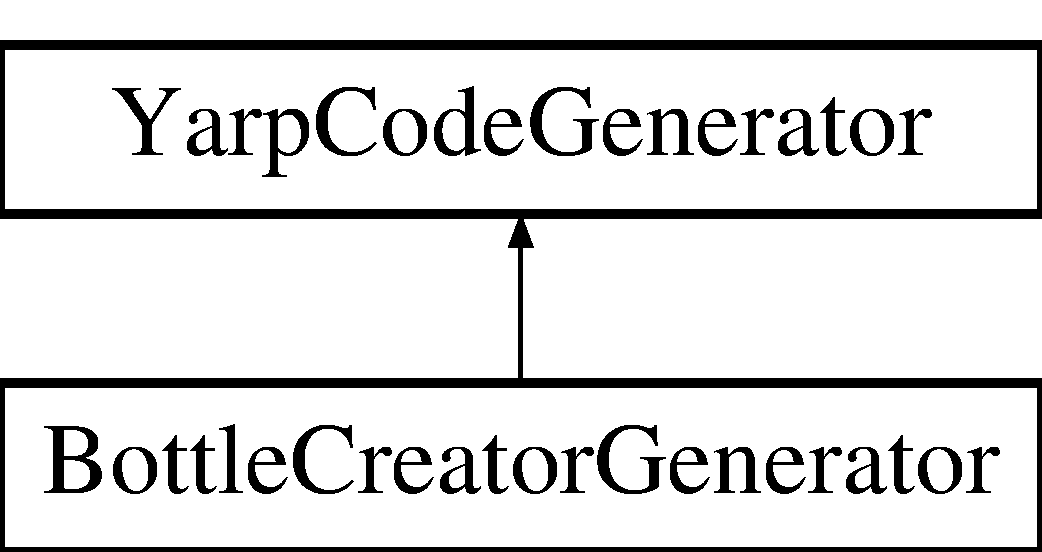
\includegraphics[height=2.000000cm]{classBottleCreatorGenerator}
\end{center}
\end{figure}
\subsection*{Public Member Functions}
\begin{DoxyCompactItemize}
\item 
\hyperlink{classBottleCreatorGenerator_a3466bff850a08d9cc93eb8b06ae945d8}{Bottle\-Creator\-Generator} (int num\-Fields, const double \&rate\-\_\-, bool to\-Ros)
\item 
\hyperlink{classBottleCreatorGenerator_a257c47964cfc58ffa7d5fcd44ae1aba4}{$\sim$\-Bottle\-Creator\-Generator} ()
\item 
\hypertarget{classBottleCreatorGenerator_a34be855391145c00dd7f3a2bb41abda5}{int {\bfseries get\-Num\-Fields} ()}\label{classBottleCreatorGenerator_a34be855391145c00dd7f3a2bb41abda5}

\item 
\hypertarget{classBottleCreatorGenerator_a93ddde67ac5b011f15d445ba6f8a84f7}{std\-::vector$<$ \hyperlink{classChildGenerator}{Child\-Generator} $>$ {\bfseries get\-Children} ()}\label{classBottleCreatorGenerator_a93ddde67ac5b011f15d445ba6f8a84f7}

\item 
\hypertarget{classBottleCreatorGenerator_af7d7eea7711f8511ddae33a51dd8b937}{std\-::vector$<$ std\-::string $>$ {\bfseries get\-Fields\-Type} ()}\label{classBottleCreatorGenerator_af7d7eea7711f8511ddae33a51dd8b937}

\item 
\hypertarget{classBottleCreatorGenerator_aa034b1338c9f0b3346e52e5bce4156ee}{std\-::vector$<$ std\-::string $>$ {\bfseries get\-Fields\-Msg} ()}\label{classBottleCreatorGenerator_aa034b1338c9f0b3346e52e5bce4156ee}

\item 
\hypertarget{classBottleCreatorGenerator_ab71bdfa8a3fa42e88453f40e82f53d4b}{std\-::vector$<$ std\-::string $>$ {\bfseries get\-Fields\-Mux} ()}\label{classBottleCreatorGenerator_ab71bdfa8a3fa42e88453f40e82f53d4b}

\item 
\hypertarget{classBottleCreatorGenerator_a57eef736e9ce07393c22f6face03b0e0}{void {\bfseries add\-Child} (\hyperlink{classChildGenerator}{Child\-Generator} \&child)}\label{classBottleCreatorGenerator_a57eef736e9ce07393c22f6face03b0e0}

\item 
\hypertarget{classBottleCreatorGenerator_ae26464fccf513247ec7b4ef1c015936d}{void {\bfseries add\-Field\-Type} (std\-::string type)}\label{classBottleCreatorGenerator_ae26464fccf513247ec7b4ef1c015936d}

\item 
\hypertarget{classBottleCreatorGenerator_aea16ec13577f661086c30bd335ad58f2}{void {\bfseries add\-Field\-Msg} (std\-::string msg)}\label{classBottleCreatorGenerator_aea16ec13577f661086c30bd335ad58f2}

\item 
\hypertarget{classBottleCreatorGenerator_ac020e7913971161859f728e40f3dc253}{void {\bfseries add\-Field\-Mux} (std\-::string mux)}\label{classBottleCreatorGenerator_ac020e7913971161859f728e40f3dc253}

\item 
\hypertarget{classBottleCreatorGenerator_a328f92df32dcdc006008c19bfb1b4c25}{void {\bfseries remove\-First\-Child} ()}\label{classBottleCreatorGenerator_a328f92df32dcdc006008c19bfb1b4c25}

\item 
\hypertarget{classBottleCreatorGenerator_aec44a986041ce21c06f9c8540fcb667d}{\hyperlink{classChildGenerator}{Child\-Generator} \& {\bfseries get\-First\-Child} ()}\label{classBottleCreatorGenerator_aec44a986041ce21c06f9c8540fcb667d}

\item 
\hypertarget{classBottleCreatorGenerator_a862b67f6ea3ac4cf43f0b32feb44e682}{std\-::string {\bfseries get\-Field\-Type} (int field\-Index)}\label{classBottleCreatorGenerator_a862b67f6ea3ac4cf43f0b32feb44e682}

\item 
\hypertarget{classBottleCreatorGenerator_aa473bc54a236b2fe7016a640343396b1}{std\-::string {\bfseries get\-Field\-Msg} (int field\-Index)}\label{classBottleCreatorGenerator_aa473bc54a236b2fe7016a640343396b1}

\item 
\hypertarget{classBottleCreatorGenerator_a1090efb927fe566d4977a613f8221368}{std\-::string {\bfseries get\-Field\-Mux} (int field\-Index)}\label{classBottleCreatorGenerator_a1090efb927fe566d4977a613f8221368}

\item 
std\-::string \hyperlink{classBottleCreatorGenerator_a71d28a76d750bcfa2de6f62f8b9b5a62}{generate\-Code} ()
\end{DoxyCompactItemize}
\subsection*{Private Member Functions}
\begin{DoxyCompactItemize}
\item 
std\-::string \hyperlink{classBottleCreatorGenerator_a691d8b9a0bc0796c4253286db7e3f1ac}{handle\-Field\-Generation} (int field\-Index)
\end{DoxyCompactItemize}
\subsection*{Private Attributes}
\begin{DoxyCompactItemize}
\item 
int \hyperlink{classBottleCreatorGenerator_ab2b5f38e2b44b14d26ca3eebcb42648a}{num\-Fields\-\_\-}
\item 
\hypertarget{classBottleCreatorGenerator_ad5c777ad4890fc3dfd9b74b67a9e0019}{int {\bfseries list\-Index\-\_\-}}\label{classBottleCreatorGenerator_ad5c777ad4890fc3dfd9b74b67a9e0019}

\item 
bool \hyperlink{classBottleCreatorGenerator_aa20440ff74cb4ee807221653872611dd}{to\-Ros\-\_\-}
\item 
std\-::vector$<$ \hyperlink{classChildGenerator}{Child\-Generator} $>$ \hyperlink{classBottleCreatorGenerator_a1e0f07071fec2afe0c6f0ec1f9324ba9}{children\-\_\-}
\item 
std\-::vector$<$ std\-::string $>$ \hyperlink{classBottleCreatorGenerator_abad8d5103182e56c2c9b96cab85c0602}{fields\-Type\-\_\-}
\item 
std\-::vector$<$ std\-::string $>$ \hyperlink{classBottleCreatorGenerator_a805fb77a1f16e0816b639ae06cbca361}{fields\-Msg\-\_\-}
\item 
std\-::vector$<$ std\-::string $>$ \hyperlink{classBottleCreatorGenerator_a5bd421cf5bc8157b46ef8d6522bc79e2}{fields\-Mux\-\_\-}
\item 
\hypertarget{classBottleCreatorGenerator_a20a7016668f375ed392d25984b732e23}{double {\bfseries rate}}\label{classBottleCreatorGenerator_a20a7016668f375ed392d25984b732e23}

\item 
\hypertarget{classBottleCreatorGenerator_a856a5521bdb4813a09f0bdfcd51354ec}{double {\bfseries period}}\label{classBottleCreatorGenerator_a856a5521bdb4813a09f0bdfcd51354ec}

\end{DoxyCompactItemize}


\subsection{Detailed Description}
Class that generates the code for building the message and sending it through the network (Y\-A\-R\-P port/\-R\-O\-S topic) This class represents the top level of the message hierarchy (root of the tree) 

Definition at line 10 of file bottlecreatorgenerator.\-hpp.



\subsection{Constructor \& Destructor Documentation}
\hypertarget{classBottleCreatorGenerator_a3466bff850a08d9cc93eb8b06ae945d8}{\index{Bottle\-Creator\-Generator@{Bottle\-Creator\-Generator}!Bottle\-Creator\-Generator@{Bottle\-Creator\-Generator}}
\index{Bottle\-Creator\-Generator@{Bottle\-Creator\-Generator}!BottleCreatorGenerator@{Bottle\-Creator\-Generator}}
\subsubsection[{Bottle\-Creator\-Generator}]{\setlength{\rightskip}{0pt plus 5cm}Bottle\-Creator\-Generator\-::\-Bottle\-Creator\-Generator (
\begin{DoxyParamCaption}
\item[{int}]{num\-Fields, }
\item[{const double \&}]{rate\-\_\-, }
\item[{bool}]{to\-Ros}
\end{DoxyParamCaption}
)}}\label{classBottleCreatorGenerator_a3466bff850a08d9cc93eb8b06ae945d8}
Constructor 
\begin{DoxyParams}{Parameters}
{\em num\-Fields} & Number of items (either simple types or messages) of the message \\
\hline
{\em rate\-\_\-} & Rate at which the message will be sent (hz) \\
\hline
{\em to\-Ros} & Boolean flag to know the type of output (R\-O\-S message or Y\-A\-R\-P Bottle) \\
\hline
\end{DoxyParams}


Definition at line 7 of file bottlecreatorgenerator.\-cpp.

\hypertarget{classBottleCreatorGenerator_a257c47964cfc58ffa7d5fcd44ae1aba4}{\index{Bottle\-Creator\-Generator@{Bottle\-Creator\-Generator}!$\sim$\-Bottle\-Creator\-Generator@{$\sim$\-Bottle\-Creator\-Generator}}
\index{$\sim$\-Bottle\-Creator\-Generator@{$\sim$\-Bottle\-Creator\-Generator}!BottleCreatorGenerator@{Bottle\-Creator\-Generator}}
\subsubsection[{$\sim$\-Bottle\-Creator\-Generator}]{\setlength{\rightskip}{0pt plus 5cm}Bottle\-Creator\-Generator\-::$\sim$\-Bottle\-Creator\-Generator (
\begin{DoxyParamCaption}
{}
\end{DoxyParamCaption}
)}}\label{classBottleCreatorGenerator_a257c47964cfc58ffa7d5fcd44ae1aba4}
Destructor 

Definition at line 16 of file bottlecreatorgenerator.\-cpp.



\subsection{Member Function Documentation}
\hypertarget{classBottleCreatorGenerator_a71d28a76d750bcfa2de6f62f8b9b5a62}{\index{Bottle\-Creator\-Generator@{Bottle\-Creator\-Generator}!generate\-Code@{generate\-Code}}
\index{generate\-Code@{generate\-Code}!BottleCreatorGenerator@{Bottle\-Creator\-Generator}}
\subsubsection[{generate\-Code}]{\setlength{\rightskip}{0pt plus 5cm}std\-::string Bottle\-Creator\-Generator\-::generate\-Code (
\begin{DoxyParamCaption}
{}
\end{DoxyParamCaption}
)\hspace{0.3cm}{\ttfamily [virtual]}}}\label{classBottleCreatorGenerator_a71d28a76d750bcfa2de6f62f8b9b5a62}
Generates the code that builds the message for all the items in the configuration file \begin{DoxyReturn}{Returns}
String that contains the code for message building and sending, considering the frequency 
\end{DoxyReturn}


Implements \hyperlink{classYarpCodeGenerator_ad4247b4dad2a694c3799d5a6968faa41}{Yarp\-Code\-Generator}.



Definition at line 76 of file bottlecreatorgenerator.\-cpp.

\hypertarget{classBottleCreatorGenerator_a691d8b9a0bc0796c4253286db7e3f1ac}{\index{Bottle\-Creator\-Generator@{Bottle\-Creator\-Generator}!handle\-Field\-Generation@{handle\-Field\-Generation}}
\index{handle\-Field\-Generation@{handle\-Field\-Generation}!BottleCreatorGenerator@{Bottle\-Creator\-Generator}}
\subsubsection[{handle\-Field\-Generation}]{\setlength{\rightskip}{0pt plus 5cm}std\-::string Bottle\-Creator\-Generator\-::handle\-Field\-Generation (
\begin{DoxyParamCaption}
\item[{int}]{field\-Index}
\end{DoxyParamCaption}
)\hspace{0.3cm}{\ttfamily [private]}}}\label{classBottleCreatorGenerator_a691d8b9a0bc0796c4253286db7e3f1ac}
Generates the code that builds the message for an item of the top of the hierarchy, considering all its children in the message tree 
\begin{DoxyParams}{Parameters}
{\em index} & at the \hyperlink{classChildGenerator}{Child\-Generator} std\-::vector \\
\hline
\end{DoxyParams}
\begin{DoxyReturn}{Returns}
String that contains the code for message building 
\end{DoxyReturn}


Definition at line 99 of file bottlecreatorgenerator.\-cpp.



\subsection{Member Data Documentation}
\hypertarget{classBottleCreatorGenerator_a1e0f07071fec2afe0c6f0ec1f9324ba9}{\index{Bottle\-Creator\-Generator@{Bottle\-Creator\-Generator}!children\-\_\-@{children\-\_\-}}
\index{children\-\_\-@{children\-\_\-}!BottleCreatorGenerator@{Bottle\-Creator\-Generator}}
\subsubsection[{children\-\_\-}]{\setlength{\rightskip}{0pt plus 5cm}std\-::vector$<${\bf Child\-Generator}$>$ Bottle\-Creator\-Generator\-::children\-\_\-\hspace{0.3cm}{\ttfamily [private]}}}\label{classBottleCreatorGenerator_a1e0f07071fec2afe0c6f0ec1f9324ba9}
Vector of \hyperlink{classChildGenerator}{Child\-Generator} class, that handles built-\/in (primitive) messages and arrays of built-\/in messages 

Definition at line 62 of file bottlecreatorgenerator.\-hpp.

\hypertarget{classBottleCreatorGenerator_a805fb77a1f16e0816b639ae06cbca361}{\index{Bottle\-Creator\-Generator@{Bottle\-Creator\-Generator}!fields\-Msg\-\_\-@{fields\-Msg\-\_\-}}
\index{fields\-Msg\-\_\-@{fields\-Msg\-\_\-}!BottleCreatorGenerator@{Bottle\-Creator\-Generator}}
\subsubsection[{fields\-Msg\-\_\-}]{\setlength{\rightskip}{0pt plus 5cm}std\-::vector$<$std\-::string$>$ Bottle\-Creator\-Generator\-::fields\-Msg\-\_\-\hspace{0.3cm}{\ttfamily [private]}}}\label{classBottleCreatorGenerator_a805fb77a1f16e0816b639ae06cbca361}
Vector of std\-::string that stores \char`\"{}single\-\_\-value\char`\"{} or \char`\"{}list\char`\"{} if that is the type of the item 

Definition at line 64 of file bottlecreatorgenerator.\-hpp.

\hypertarget{classBottleCreatorGenerator_a5bd421cf5bc8157b46ef8d6522bc79e2}{\index{Bottle\-Creator\-Generator@{Bottle\-Creator\-Generator}!fields\-Mux\-\_\-@{fields\-Mux\-\_\-}}
\index{fields\-Mux\-\_\-@{fields\-Mux\-\_\-}!BottleCreatorGenerator@{Bottle\-Creator\-Generator}}
\subsubsection[{fields\-Mux\-\_\-}]{\setlength{\rightskip}{0pt plus 5cm}std\-::vector$<$std\-::string$>$ Bottle\-Creator\-Generator\-::fields\-Mux\-\_\-\hspace{0.3cm}{\ttfamily [private]}}}\label{classBottleCreatorGenerator_a5bd421cf5bc8157b46ef8d6522bc79e2}
Vector of std\-::string that stores \char`\"{}mux\char`\"{} if that is the type of the item 

Definition at line 65 of file bottlecreatorgenerator.\-hpp.

\hypertarget{classBottleCreatorGenerator_abad8d5103182e56c2c9b96cab85c0602}{\index{Bottle\-Creator\-Generator@{Bottle\-Creator\-Generator}!fields\-Type\-\_\-@{fields\-Type\-\_\-}}
\index{fields\-Type\-\_\-@{fields\-Type\-\_\-}!BottleCreatorGenerator@{Bottle\-Creator\-Generator}}
\subsubsection[{fields\-Type\-\_\-}]{\setlength{\rightskip}{0pt plus 5cm}std\-::vector$<$std\-::string$>$ Bottle\-Creator\-Generator\-::fields\-Type\-\_\-\hspace{0.3cm}{\ttfamily [private]}}}\label{classBottleCreatorGenerator_abad8d5103182e56c2c9b96cab85c0602}
Vector of std\-::string that contains all the message types at the top of the message hierarchy, read from the configuration file 

Definition at line 63 of file bottlecreatorgenerator.\-hpp.

\hypertarget{classBottleCreatorGenerator_ab2b5f38e2b44b14d26ca3eebcb42648a}{\index{Bottle\-Creator\-Generator@{Bottle\-Creator\-Generator}!num\-Fields\-\_\-@{num\-Fields\-\_\-}}
\index{num\-Fields\-\_\-@{num\-Fields\-\_\-}!BottleCreatorGenerator@{Bottle\-Creator\-Generator}}
\subsubsection[{num\-Fields\-\_\-}]{\setlength{\rightskip}{0pt plus 5cm}int Bottle\-Creator\-Generator\-::num\-Fields\-\_\-\hspace{0.3cm}{\ttfamily [private]}}}\label{classBottleCreatorGenerator_ab2b5f38e2b44b14d26ca3eebcb42648a}
Number of items in the message 

Definition at line 59 of file bottlecreatorgenerator.\-hpp.

\hypertarget{classBottleCreatorGenerator_aa20440ff74cb4ee807221653872611dd}{\index{Bottle\-Creator\-Generator@{Bottle\-Creator\-Generator}!to\-Ros\-\_\-@{to\-Ros\-\_\-}}
\index{to\-Ros\-\_\-@{to\-Ros\-\_\-}!BottleCreatorGenerator@{Bottle\-Creator\-Generator}}
\subsubsection[{to\-Ros\-\_\-}]{\setlength{\rightskip}{0pt plus 5cm}bool Bottle\-Creator\-Generator\-::to\-Ros\-\_\-\hspace{0.3cm}{\ttfamily [private]}}}\label{classBottleCreatorGenerator_aa20440ff74cb4ee807221653872611dd}
Boolean flag to know the type of output 

Definition at line 61 of file bottlecreatorgenerator.\-hpp.



The documentation for this class was generated from the following files\-:\begin{DoxyCompactItemize}
\item 
bottlecreatorgenerator.\-hpp\item 
bottlecreatorgenerator.\-cpp\end{DoxyCompactItemize}

\hypertarget{classChildGenerator}{\section{Child\-Generator Class Reference}
\label{classChildGenerator}\index{Child\-Generator@{Child\-Generator}}
}


{\ttfamily \#include $<$childgenerator.\-hpp$>$}

Inheritance diagram for Child\-Generator\-:\begin{figure}[H]
\begin{center}
\leavevmode
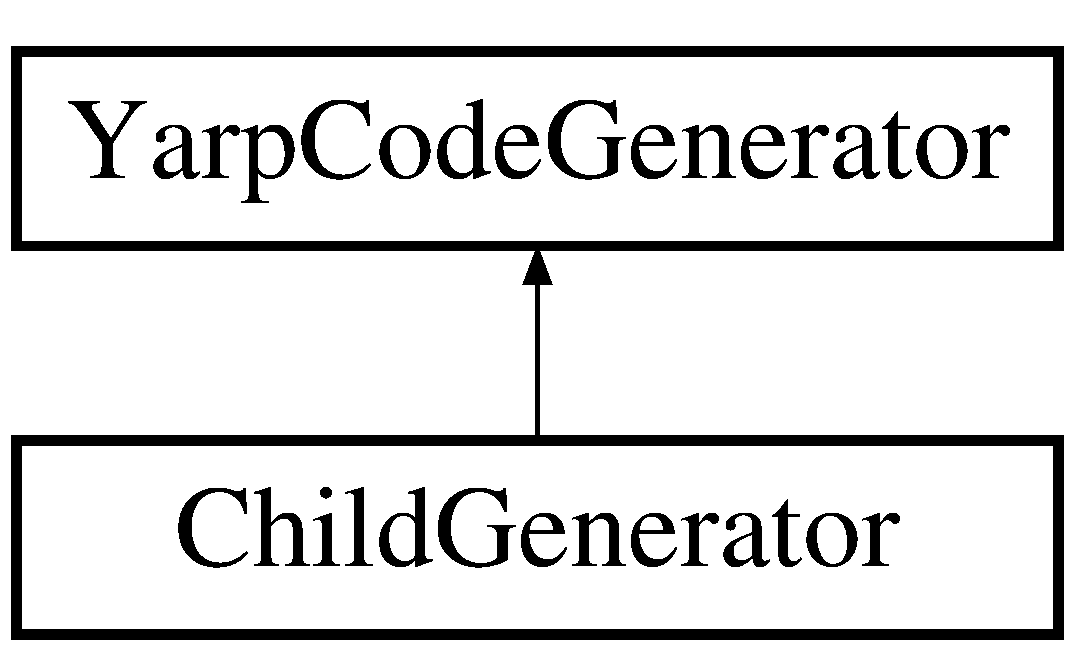
\includegraphics[height=2.000000cm]{classChildGenerator}
\end{center}
\end{figure}
\subsection*{Public Member Functions}
\begin{DoxyCompactItemize}
\item 
\hyperlink{classChildGenerator_ae32dcca9e5fdf68591c0234ac5892efb}{Child\-Generator} (int num\-Fields, bool to\-Ros)
\item 
\hyperlink{classChildGenerator_ae02e5d64e580bb25b590ca7558efaa0a}{$\sim$\-Child\-Generator} ()
\item 
\hypertarget{classChildGenerator_ae6581386da55d6cd9792fd0eb0715442}{int {\bfseries get\-Num\-Fields} ()}\label{classChildGenerator_ae6581386da55d6cd9792fd0eb0715442}

\item 
\hypertarget{classChildGenerator_a92c28e7e0312810f1db1302737c3a4f6}{std\-::vector$<$ \hyperlink{classChildGenerator}{Child\-Generator} $>$ {\bfseries get\-Children} ()}\label{classChildGenerator_a92c28e7e0312810f1db1302737c3a4f6}

\item 
\hypertarget{classChildGenerator_a5ec4534067ff985b052273f69db8b4af}{std\-::vector$<$ std\-::string $>$ {\bfseries get\-Fields\-Type} ()}\label{classChildGenerator_a5ec4534067ff985b052273f69db8b4af}

\item 
\hypertarget{classChildGenerator_aabc717278731ef281f8015b94a529786}{std\-::vector$<$ std\-::string $>$ {\bfseries get\-Fields\-Msg} ()}\label{classChildGenerator_aabc717278731ef281f8015b94a529786}

\item 
\hypertarget{classChildGenerator_a3457cb5b97dfea562dfa0dd64c5dcbeb}{std\-::vector$<$ std\-::string $>$ {\bfseries get\-Fields\-Mux} ()}\label{classChildGenerator_a3457cb5b97dfea562dfa0dd64c5dcbeb}

\item 
\hypertarget{classChildGenerator_af5f270a920e3ca8b67d6a055552fd9f8}{void {\bfseries set\-Parent\-Name} (std\-::string parent\-Name)}\label{classChildGenerator_af5f270a920e3ca8b67d6a055552fd9f8}

\item 
\hypertarget{classChildGenerator_a89df978421779b69ac49ce1ca005dd07}{void {\bfseries add\-Child} (\hyperlink{classChildGenerator}{Child\-Generator} \&child)}\label{classChildGenerator_a89df978421779b69ac49ce1ca005dd07}

\item 
\hypertarget{classChildGenerator_aa651c4d61b61b4e4db9061256996026c}{void {\bfseries add\-Field\-Type} (std\-::string type)}\label{classChildGenerator_aa651c4d61b61b4e4db9061256996026c}

\item 
\hypertarget{classChildGenerator_a4f250d173bc5495679e0bf50b6b9bfd0}{void {\bfseries add\-Field\-Msg} (std\-::string msg)}\label{classChildGenerator_a4f250d173bc5495679e0bf50b6b9bfd0}

\item 
\hypertarget{classChildGenerator_a8e6cfd5d9573009475a1154d979e8e59}{void {\bfseries add\-Field\-Mux} (std\-::string mux)}\label{classChildGenerator_a8e6cfd5d9573009475a1154d979e8e59}

\item 
\hypertarget{classChildGenerator_a52e17e0807904531c7d74c3312c419c0}{void {\bfseries remove\-First\-Child} ()}\label{classChildGenerator_a52e17e0807904531c7d74c3312c419c0}

\item 
\hypertarget{classChildGenerator_aac1dd1a96778db140c1a4c60df40608b}{\hyperlink{classChildGenerator}{Child\-Generator} \& {\bfseries get\-First\-Child} ()}\label{classChildGenerator_aac1dd1a96778db140c1a4c60df40608b}

\item 
\hypertarget{classChildGenerator_aafdee6300b9422ce5521655bcd7ccb9f}{std\-::string {\bfseries get\-Field\-Type} (int field\-Index)}\label{classChildGenerator_aafdee6300b9422ce5521655bcd7ccb9f}

\item 
\hypertarget{classChildGenerator_ac2d36434a7f395b245f7e0719b5cba6b}{std\-::string {\bfseries get\-Field\-Msg} (int field\-Index)}\label{classChildGenerator_ac2d36434a7f395b245f7e0719b5cba6b}

\item 
\hypertarget{classChildGenerator_af05c7bf865614b4e047737969f1bf2ab}{std\-::string {\bfseries get\-Field\-Mux} (int field\-Index)}\label{classChildGenerator_af05c7bf865614b4e047737969f1bf2ab}

\item 
std\-::string \hyperlink{classChildGenerator_a2dd3b214edfe346d16c8c2cdc708cc52}{generate\-Code} ()
\end{DoxyCompactItemize}
\subsection*{Private Member Functions}
\begin{DoxyCompactItemize}
\item 
std\-::string \hyperlink{classChildGenerator_a714d69356bb97be6914758a8d5c7636c}{handle\-Field\-Generation} (int field\-Index)
\end{DoxyCompactItemize}
\subsection*{Private Attributes}
\begin{DoxyCompactItemize}
\item 
int \hyperlink{classChildGenerator_ad485f88e3559a3643c700f8c39e76035}{num\-Fields\-\_\-}
\item 
bool \hyperlink{classChildGenerator_a7b1a36a6a5679fbd2d54682b6cb0527b}{to\-Ros\-\_\-}
\item 
\hypertarget{classChildGenerator_a2d90e8fefb81ef4eb34c7d114e23baae}{int {\bfseries list\-Index\-\_\-}}\label{classChildGenerator_a2d90e8fefb81ef4eb34c7d114e23baae}

\item 
\hypertarget{classChildGenerator_a7958558445170f12ee568c7b3c730b4b}{std\-::string {\bfseries parent\-Name\-\_\-}}\label{classChildGenerator_a7958558445170f12ee568c7b3c730b4b}

\item 
std\-::vector$<$ \hyperlink{classChildGenerator}{Child\-Generator} $>$ \hyperlink{classChildGenerator_ab54bc0742dc6acaf310afb296a154a96}{children\-\_\-}
\item 
std\-::vector$<$ std\-::string $>$ \hyperlink{classChildGenerator_a410cf2b350df1977ac4679bb608859cf}{fields\-Type\-\_\-}
\item 
std\-::vector$<$ std\-::string $>$ \hyperlink{classChildGenerator_a6e4d1e3a323027b3e4277b385b483688}{fields\-Msg\-\_\-}
\item 
std\-::vector$<$ std\-::string $>$ \hyperlink{classChildGenerator_aeb69f47a9b38b931c8c8fdef61d0a4eb}{fields\-Mux\-\_\-}
\end{DoxyCompactItemize}


\subsection{Detailed Description}
Class that generates the code for building the message and sending it through the network (Y\-A\-R\-P port/\-R\-O\-S topic) This class represents the any leaf of the message hierarchy (not the root of the tree) 

Definition at line 9 of file childgenerator.\-hpp.



\subsection{Constructor \& Destructor Documentation}
\hypertarget{classChildGenerator_ae32dcca9e5fdf68591c0234ac5892efb}{\index{Child\-Generator@{Child\-Generator}!Child\-Generator@{Child\-Generator}}
\index{Child\-Generator@{Child\-Generator}!ChildGenerator@{Child\-Generator}}
\subsubsection[{Child\-Generator}]{\setlength{\rightskip}{0pt plus 5cm}Child\-Generator\-::\-Child\-Generator (
\begin{DoxyParamCaption}
\item[{int}]{num\-Fields, }
\item[{bool}]{to\-Ros}
\end{DoxyParamCaption}
)}}\label{classChildGenerator_ae32dcca9e5fdf68591c0234ac5892efb}
Constructor 
\begin{DoxyParams}{Parameters}
{\em num\-Fields} & Number of items (either simple types or messages) of the message \\
\hline
{\em to\-Ros} & Boolean flag to know the type of output (R\-O\-S message or Y\-A\-R\-P Bottle) \\
\hline
\end{DoxyParams}


Definition at line 8 of file childgenerator.\-cpp.

\hypertarget{classChildGenerator_ae02e5d64e580bb25b590ca7558efaa0a}{\index{Child\-Generator@{Child\-Generator}!$\sim$\-Child\-Generator@{$\sim$\-Child\-Generator}}
\index{$\sim$\-Child\-Generator@{$\sim$\-Child\-Generator}!ChildGenerator@{Child\-Generator}}
\subsubsection[{$\sim$\-Child\-Generator}]{\setlength{\rightskip}{0pt plus 5cm}Child\-Generator\-::$\sim$\-Child\-Generator (
\begin{DoxyParamCaption}
{}
\end{DoxyParamCaption}
)}}\label{classChildGenerator_ae02e5d64e580bb25b590ca7558efaa0a}
Destructor 

Definition at line 13 of file childgenerator.\-cpp.



\subsection{Member Function Documentation}
\hypertarget{classChildGenerator_a2dd3b214edfe346d16c8c2cdc708cc52}{\index{Child\-Generator@{Child\-Generator}!generate\-Code@{generate\-Code}}
\index{generate\-Code@{generate\-Code}!ChildGenerator@{Child\-Generator}}
\subsubsection[{generate\-Code}]{\setlength{\rightskip}{0pt plus 5cm}std\-::string Child\-Generator\-::generate\-Code (
\begin{DoxyParamCaption}
{}
\end{DoxyParamCaption}
)\hspace{0.3cm}{\ttfamily [virtual]}}}\label{classChildGenerator_a2dd3b214edfe346d16c8c2cdc708cc52}
Generates the code that builds the message for the current node in the message hierarchy and all its leaves \begin{DoxyReturn}{Returns}
String that contains the code for message building and sending 
\end{DoxyReturn}


Implements \hyperlink{classYarpCodeGenerator_ad4247b4dad2a694c3799d5a6968faa41}{Yarp\-Code\-Generator}.



Definition at line 77 of file childgenerator.\-cpp.

\hypertarget{classChildGenerator_a714d69356bb97be6914758a8d5c7636c}{\index{Child\-Generator@{Child\-Generator}!handle\-Field\-Generation@{handle\-Field\-Generation}}
\index{handle\-Field\-Generation@{handle\-Field\-Generation}!ChildGenerator@{Child\-Generator}}
\subsubsection[{handle\-Field\-Generation}]{\setlength{\rightskip}{0pt plus 5cm}std\-::string Child\-Generator\-::handle\-Field\-Generation (
\begin{DoxyParamCaption}
\item[{int}]{field\-Index}
\end{DoxyParamCaption}
)\hspace{0.3cm}{\ttfamily [private]}}}\label{classChildGenerator_a714d69356bb97be6914758a8d5c7636c}
Generates the code that builds the message for the current node in the hierarchy, considering all its children in the tree 
\begin{DoxyParams}{Parameters}
{\em index} & at the \hyperlink{classChildGenerator}{Child\-Generator} std\-::vector \\
\hline
\end{DoxyParams}
\begin{DoxyReturn}{Returns}
String that contains the code for message building 
\end{DoxyReturn}


Definition at line 87 of file childgenerator.\-cpp.



\subsection{Member Data Documentation}
\hypertarget{classChildGenerator_ab54bc0742dc6acaf310afb296a154a96}{\index{Child\-Generator@{Child\-Generator}!children\-\_\-@{children\-\_\-}}
\index{children\-\_\-@{children\-\_\-}!ChildGenerator@{Child\-Generator}}
\subsubsection[{children\-\_\-}]{\setlength{\rightskip}{0pt plus 5cm}std\-::vector$<${\bf Child\-Generator}$>$ Child\-Generator\-::children\-\_\-\hspace{0.3cm}{\ttfamily [private]}}}\label{classChildGenerator_ab54bc0742dc6acaf310afb296a154a96}
Vector of \hyperlink{classChildGenerator}{Child\-Generator} class, that handles built-\/in (primitive) messages and arrays of built-\/in messages 

Definition at line 63 of file childgenerator.\-hpp.

\hypertarget{classChildGenerator_a6e4d1e3a323027b3e4277b385b483688}{\index{Child\-Generator@{Child\-Generator}!fields\-Msg\-\_\-@{fields\-Msg\-\_\-}}
\index{fields\-Msg\-\_\-@{fields\-Msg\-\_\-}!ChildGenerator@{Child\-Generator}}
\subsubsection[{fields\-Msg\-\_\-}]{\setlength{\rightskip}{0pt plus 5cm}std\-::vector$<$std\-::string$>$ Child\-Generator\-::fields\-Msg\-\_\-\hspace{0.3cm}{\ttfamily [private]}}}\label{classChildGenerator_a6e4d1e3a323027b3e4277b385b483688}
Vector of std\-::string that stores \char`\"{}single\-\_\-value\char`\"{} or \char`\"{}list\char`\"{} if that is the type of the item 

Definition at line 65 of file childgenerator.\-hpp.

\hypertarget{classChildGenerator_aeb69f47a9b38b931c8c8fdef61d0a4eb}{\index{Child\-Generator@{Child\-Generator}!fields\-Mux\-\_\-@{fields\-Mux\-\_\-}}
\index{fields\-Mux\-\_\-@{fields\-Mux\-\_\-}!ChildGenerator@{Child\-Generator}}
\subsubsection[{fields\-Mux\-\_\-}]{\setlength{\rightskip}{0pt plus 5cm}std\-::vector$<$std\-::string$>$ Child\-Generator\-::fields\-Mux\-\_\-\hspace{0.3cm}{\ttfamily [private]}}}\label{classChildGenerator_aeb69f47a9b38b931c8c8fdef61d0a4eb}
Vector of std\-::string that stores \char`\"{}mux\char`\"{} if that is the type of the item 

Definition at line 66 of file childgenerator.\-hpp.

\hypertarget{classChildGenerator_a410cf2b350df1977ac4679bb608859cf}{\index{Child\-Generator@{Child\-Generator}!fields\-Type\-\_\-@{fields\-Type\-\_\-}}
\index{fields\-Type\-\_\-@{fields\-Type\-\_\-}!ChildGenerator@{Child\-Generator}}
\subsubsection[{fields\-Type\-\_\-}]{\setlength{\rightskip}{0pt plus 5cm}std\-::vector$<$std\-::string$>$ Child\-Generator\-::fields\-Type\-\_\-\hspace{0.3cm}{\ttfamily [private]}}}\label{classChildGenerator_a410cf2b350df1977ac4679bb608859cf}
Vector of std\-::string that contains all the message types at the current node in the message hierarchy, read from the configuration file 

Definition at line 64 of file childgenerator.\-hpp.

\hypertarget{classChildGenerator_ad485f88e3559a3643c700f8c39e76035}{\index{Child\-Generator@{Child\-Generator}!num\-Fields\-\_\-@{num\-Fields\-\_\-}}
\index{num\-Fields\-\_\-@{num\-Fields\-\_\-}!ChildGenerator@{Child\-Generator}}
\subsubsection[{num\-Fields\-\_\-}]{\setlength{\rightskip}{0pt plus 5cm}int Child\-Generator\-::num\-Fields\-\_\-\hspace{0.3cm}{\ttfamily [private]}}}\label{classChildGenerator_ad485f88e3559a3643c700f8c39e76035}
Number of items in the current node 

Definition at line 59 of file childgenerator.\-hpp.

\hypertarget{classChildGenerator_a7b1a36a6a5679fbd2d54682b6cb0527b}{\index{Child\-Generator@{Child\-Generator}!to\-Ros\-\_\-@{to\-Ros\-\_\-}}
\index{to\-Ros\-\_\-@{to\-Ros\-\_\-}!ChildGenerator@{Child\-Generator}}
\subsubsection[{to\-Ros\-\_\-}]{\setlength{\rightskip}{0pt plus 5cm}bool Child\-Generator\-::to\-Ros\-\_\-\hspace{0.3cm}{\ttfamily [private]}}}\label{classChildGenerator_a7b1a36a6a5679fbd2d54682b6cb0527b}
Boolean flag to know the type of output 

Definition at line 60 of file childgenerator.\-hpp.



The documentation for this class was generated from the following files\-:\begin{DoxyCompactItemize}
\item 
childgenerator.\-hpp\item 
childgenerator.\-cpp\end{DoxyCompactItemize}

\hypertarget{classCMakeFileGenerator}{\section{C\-Make\-File\-Generator Class Reference}
\label{classCMakeFileGenerator}\index{C\-Make\-File\-Generator@{C\-Make\-File\-Generator}}
}


{\ttfamily \#include $<$cmakefilegenerator.\-hpp$>$}

Inheritance diagram for C\-Make\-File\-Generator\-:\begin{figure}[H]
\begin{center}
\leavevmode
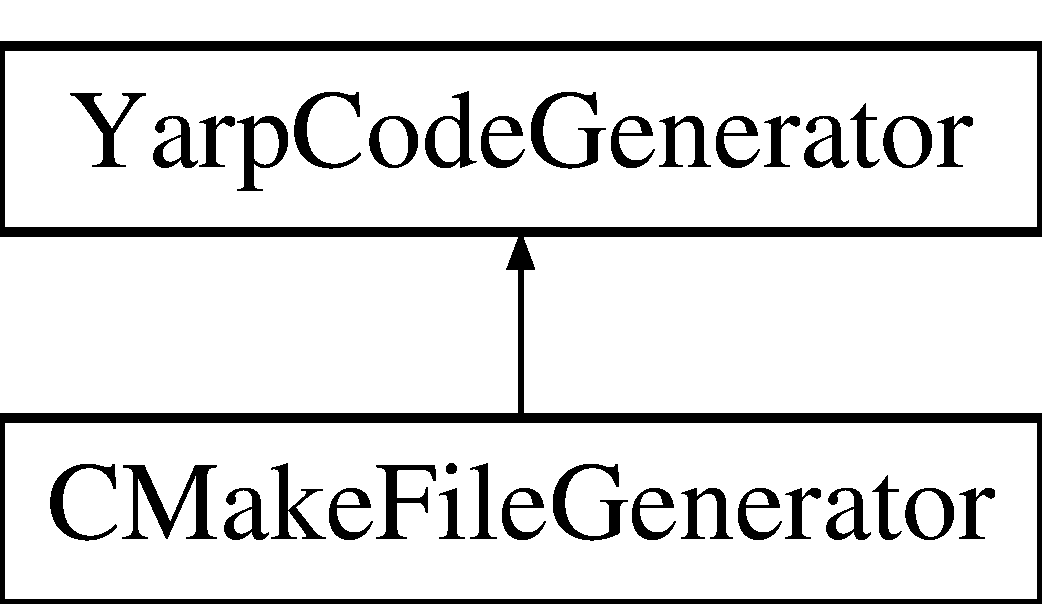
\includegraphics[height=2.000000cm]{classCMakeFileGenerator}
\end{center}
\end{figure}
\subsection*{Public Member Functions}
\begin{DoxyCompactItemize}
\item 
\hyperlink{classCMakeFileGenerator_ae32699b494f3da614136b0fb98b4b7ed}{C\-Make\-File\-Generator} ()
\item 
\hyperlink{classCMakeFileGenerator_a80fd5243000f1129a1daccd82293c4b6}{$\sim$\-C\-Make\-File\-Generator} ()
\item 
std\-::string \hyperlink{classCMakeFileGenerator_a5505ce5e4f9397e616f521e70f56f9d7}{generate\-Code} ()
\end{DoxyCompactItemize}
\subsection*{Public Attributes}
\begin{DoxyCompactItemize}
\item 
\hypertarget{classCMakeFileGenerator_a9d208171c647b3f70ae7131b670e2a32}{std\-::string {\bfseries cpp\-\_\-file\-\_\-name}}\label{classCMakeFileGenerator_a9d208171c647b3f70ae7131b670e2a32}

\end{DoxyCompactItemize}


\subsection{Detailed Description}
Class that generates the text of the C\-Make\-Lists.\-txt file 

Definition at line 9 of file cmakefilegenerator.\-hpp.



\subsection{Constructor \& Destructor Documentation}
\hypertarget{classCMakeFileGenerator_ae32699b494f3da614136b0fb98b4b7ed}{\index{C\-Make\-File\-Generator@{C\-Make\-File\-Generator}!C\-Make\-File\-Generator@{C\-Make\-File\-Generator}}
\index{C\-Make\-File\-Generator@{C\-Make\-File\-Generator}!CMakeFileGenerator@{C\-Make\-File\-Generator}}
\subsubsection[{C\-Make\-File\-Generator}]{\setlength{\rightskip}{0pt plus 5cm}C\-Make\-File\-Generator\-::\-C\-Make\-File\-Generator (
\begin{DoxyParamCaption}
{}
\end{DoxyParamCaption}
)}}\label{classCMakeFileGenerator_ae32699b494f3da614136b0fb98b4b7ed}
Constructor 

Definition at line 6 of file cmakefilegenerator.\-cpp.

\hypertarget{classCMakeFileGenerator_a80fd5243000f1129a1daccd82293c4b6}{\index{C\-Make\-File\-Generator@{C\-Make\-File\-Generator}!$\sim$\-C\-Make\-File\-Generator@{$\sim$\-C\-Make\-File\-Generator}}
\index{$\sim$\-C\-Make\-File\-Generator@{$\sim$\-C\-Make\-File\-Generator}!CMakeFileGenerator@{C\-Make\-File\-Generator}}
\subsubsection[{$\sim$\-C\-Make\-File\-Generator}]{\setlength{\rightskip}{0pt plus 5cm}C\-Make\-File\-Generator\-::$\sim$\-C\-Make\-File\-Generator (
\begin{DoxyParamCaption}
{}
\end{DoxyParamCaption}
)}}\label{classCMakeFileGenerator_a80fd5243000f1129a1daccd82293c4b6}
Destructor 

Definition at line 10 of file cmakefilegenerator.\-cpp.



\subsection{Member Function Documentation}
\hypertarget{classCMakeFileGenerator_a5505ce5e4f9397e616f521e70f56f9d7}{\index{C\-Make\-File\-Generator@{C\-Make\-File\-Generator}!generate\-Code@{generate\-Code}}
\index{generate\-Code@{generate\-Code}!CMakeFileGenerator@{C\-Make\-File\-Generator}}
\subsubsection[{generate\-Code}]{\setlength{\rightskip}{0pt plus 5cm}std\-::string C\-Make\-File\-Generator\-::generate\-Code (
\begin{DoxyParamCaption}
{}
\end{DoxyParamCaption}
)\hspace{0.3cm}{\ttfamily [virtual]}}}\label{classCMakeFileGenerator_a5505ce5e4f9397e616f521e70f56f9d7}
Generates the C\-Make\-Lists.\-txt \begin{DoxyReturn}{Returns}
String that contains the cmake script 
\end{DoxyReturn}


Implements \hyperlink{classYarpCodeGenerator_ad4247b4dad2a694c3799d5a6968faa41}{Yarp\-Code\-Generator}.



Definition at line 14 of file cmakefilegenerator.\-cpp.



The documentation for this class was generated from the following files\-:\begin{DoxyCompactItemize}
\item 
cmakefilegenerator.\-hpp\item 
cmakefilegenerator.\-cpp\end{DoxyCompactItemize}

\hypertarget{classCommonBeginningGenerator}{\section{Common\-Beginning\-Generator Class Reference}
\label{classCommonBeginningGenerator}\index{Common\-Beginning\-Generator@{Common\-Beginning\-Generator}}
}


{\ttfamily \#include $<$commonbeginninggenerator.\-hpp$>$}

Inheritance diagram for Common\-Beginning\-Generator\-:\begin{figure}[H]
\begin{center}
\leavevmode
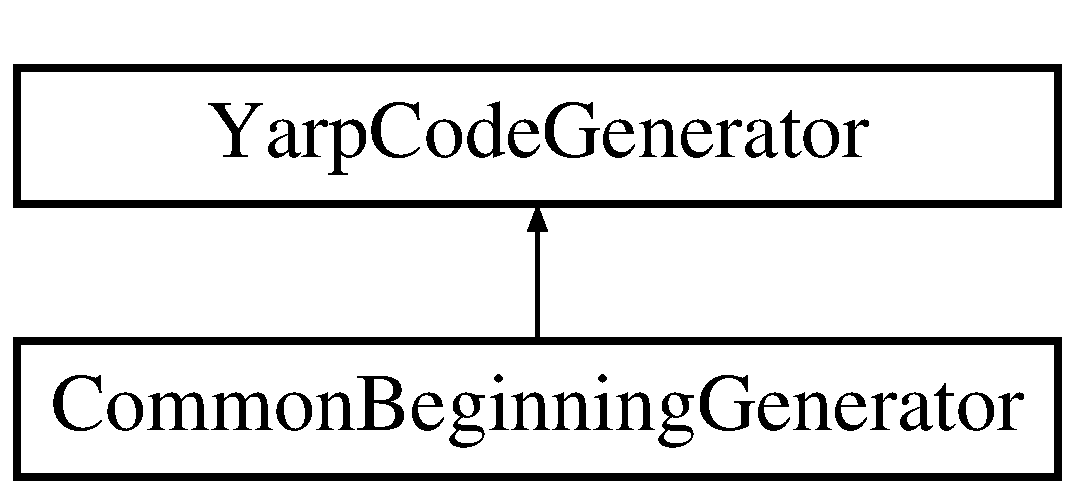
\includegraphics[height=2.000000cm]{classCommonBeginningGenerator}
\end{center}
\end{figure}
\subsection*{Public Member Functions}
\begin{DoxyCompactItemize}
\item 
\hyperlink{classCommonBeginningGenerator_a2a0e7ef7e1979ac0c6ecb789e783ef15}{Common\-Beginning\-Generator} ()
\item 
\hyperlink{classCommonBeginningGenerator_ad3be7ea31481fe1c235c0803cb967ba9}{$\sim$\-Common\-Beginning\-Generator} ()
\item 
std\-::string \hyperlink{classCommonBeginningGenerator_a34d951b06ae3658659b2c76e3bbb1413}{generate\-Code} ()
\end{DoxyCompactItemize}


\subsection{Detailed Description}
Class that generates the text of the include headers and the main function 

Definition at line 8 of file commonbeginninggenerator.\-hpp.



\subsection{Constructor \& Destructor Documentation}
\hypertarget{classCommonBeginningGenerator_a2a0e7ef7e1979ac0c6ecb789e783ef15}{\index{Common\-Beginning\-Generator@{Common\-Beginning\-Generator}!Common\-Beginning\-Generator@{Common\-Beginning\-Generator}}
\index{Common\-Beginning\-Generator@{Common\-Beginning\-Generator}!CommonBeginningGenerator@{Common\-Beginning\-Generator}}
\subsubsection[{Common\-Beginning\-Generator}]{\setlength{\rightskip}{0pt plus 5cm}Common\-Beginning\-Generator\-::\-Common\-Beginning\-Generator (
\begin{DoxyParamCaption}
{}
\end{DoxyParamCaption}
)}}\label{classCommonBeginningGenerator_a2a0e7ef7e1979ac0c6ecb789e783ef15}
Constructor 

Definition at line 5 of file commonbeginninggenerator.\-cpp.

\hypertarget{classCommonBeginningGenerator_ad3be7ea31481fe1c235c0803cb967ba9}{\index{Common\-Beginning\-Generator@{Common\-Beginning\-Generator}!$\sim$\-Common\-Beginning\-Generator@{$\sim$\-Common\-Beginning\-Generator}}
\index{$\sim$\-Common\-Beginning\-Generator@{$\sim$\-Common\-Beginning\-Generator}!CommonBeginningGenerator@{Common\-Beginning\-Generator}}
\subsubsection[{$\sim$\-Common\-Beginning\-Generator}]{\setlength{\rightskip}{0pt plus 5cm}Common\-Beginning\-Generator\-::$\sim$\-Common\-Beginning\-Generator (
\begin{DoxyParamCaption}
{}
\end{DoxyParamCaption}
)}}\label{classCommonBeginningGenerator_ad3be7ea31481fe1c235c0803cb967ba9}
Destructor 

Definition at line 9 of file commonbeginninggenerator.\-cpp.



\subsection{Member Function Documentation}
\hypertarget{classCommonBeginningGenerator_a34d951b06ae3658659b2c76e3bbb1413}{\index{Common\-Beginning\-Generator@{Common\-Beginning\-Generator}!generate\-Code@{generate\-Code}}
\index{generate\-Code@{generate\-Code}!CommonBeginningGenerator@{Common\-Beginning\-Generator}}
\subsubsection[{generate\-Code}]{\setlength{\rightskip}{0pt plus 5cm}std\-::string Common\-Beginning\-Generator\-::generate\-Code (
\begin{DoxyParamCaption}
{}
\end{DoxyParamCaption}
)\hspace{0.3cm}{\ttfamily [virtual]}}}\label{classCommonBeginningGenerator_a34d951b06ae3658659b2c76e3bbb1413}
Generates the top part of the main file \begin{DoxyReturn}{Returns}
String that contains the include headers and main function 
\end{DoxyReturn}


Implements \hyperlink{classYarpCodeGenerator_ad4247b4dad2a694c3799d5a6968faa41}{Yarp\-Code\-Generator}.



Definition at line 13 of file commonbeginninggenerator.\-cpp.



The documentation for this class was generated from the following files\-:\begin{DoxyCompactItemize}
\item 
commonbeginninggenerator.\-hpp\item 
commonbeginninggenerator.\-cpp\end{DoxyCompactItemize}

\hypertarget{classCommonEndGenerator}{\section{Common\-End\-Generator Class Reference}
\label{classCommonEndGenerator}\index{Common\-End\-Generator@{Common\-End\-Generator}}
}
Inheritance diagram for Common\-End\-Generator\-:\begin{figure}[H]
\begin{center}
\leavevmode
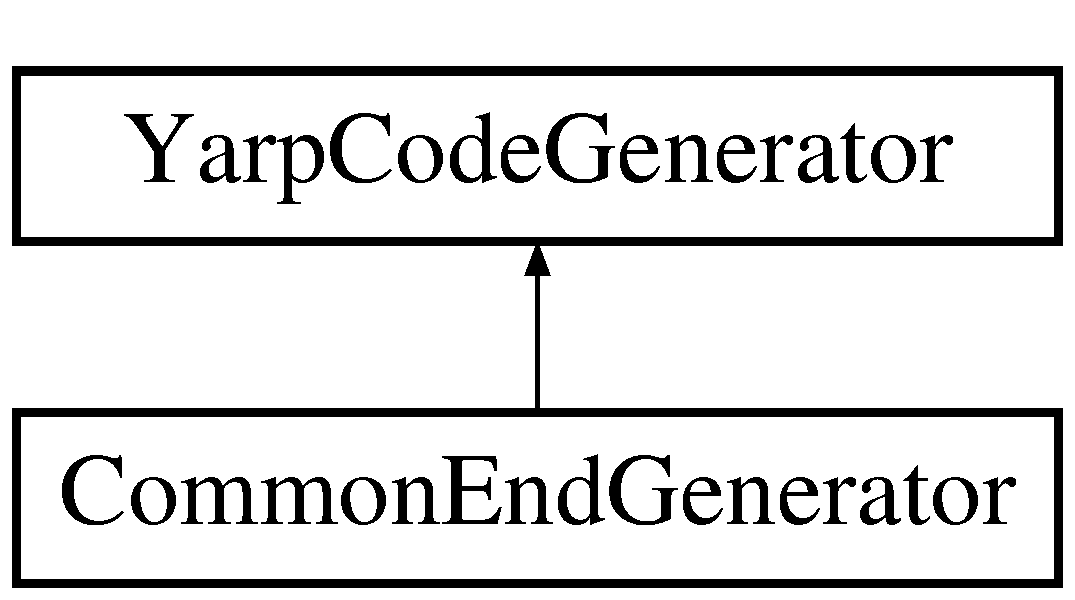
\includegraphics[height=2.000000cm]{classCommonEndGenerator}
\end{center}
\end{figure}
\subsection*{Public Member Functions}
\begin{DoxyCompactItemize}
\item 
\hyperlink{classCommonEndGenerator_a550f3eb146fac53cb8e872e6d2a9acb9}{Common\-End\-Generator} ()
\item 
\hyperlink{classCommonEndGenerator_a1a757019ff0884bd443583160aa79679}{$\sim$\-Common\-End\-Generator} ()
\item 
std\-::string \hyperlink{classCommonEndGenerator_a08904bf31bed7b708155b354ab33e272}{generate\-Code} ()
\end{DoxyCompactItemize}


\subsection{Detailed Description}


Definition at line 5 of file commonendgenerator.\-hpp.



\subsection{Constructor \& Destructor Documentation}
\hypertarget{classCommonEndGenerator_a550f3eb146fac53cb8e872e6d2a9acb9}{\index{Common\-End\-Generator@{Common\-End\-Generator}!Common\-End\-Generator@{Common\-End\-Generator}}
\index{Common\-End\-Generator@{Common\-End\-Generator}!CommonEndGenerator@{Common\-End\-Generator}}
\subsubsection[{Common\-End\-Generator}]{\setlength{\rightskip}{0pt plus 5cm}Common\-End\-Generator\-::\-Common\-End\-Generator (
\begin{DoxyParamCaption}
{}
\end{DoxyParamCaption}
)}}\label{classCommonEndGenerator_a550f3eb146fac53cb8e872e6d2a9acb9}
Constructor 

Definition at line 5 of file commonendgenerator.\-cpp.

\hypertarget{classCommonEndGenerator_a1a757019ff0884bd443583160aa79679}{\index{Common\-End\-Generator@{Common\-End\-Generator}!$\sim$\-Common\-End\-Generator@{$\sim$\-Common\-End\-Generator}}
\index{$\sim$\-Common\-End\-Generator@{$\sim$\-Common\-End\-Generator}!CommonEndGenerator@{Common\-End\-Generator}}
\subsubsection[{$\sim$\-Common\-End\-Generator}]{\setlength{\rightskip}{0pt plus 5cm}Common\-End\-Generator\-::$\sim$\-Common\-End\-Generator (
\begin{DoxyParamCaption}
{}
\end{DoxyParamCaption}
)}}\label{classCommonEndGenerator_a1a757019ff0884bd443583160aa79679}
Destructor 

Definition at line 9 of file commonendgenerator.\-cpp.



\subsection{Member Function Documentation}
\hypertarget{classCommonEndGenerator_a08904bf31bed7b708155b354ab33e272}{\index{Common\-End\-Generator@{Common\-End\-Generator}!generate\-Code@{generate\-Code}}
\index{generate\-Code@{generate\-Code}!CommonEndGenerator@{Common\-End\-Generator}}
\subsubsection[{generate\-Code}]{\setlength{\rightskip}{0pt plus 5cm}std\-::string Common\-End\-Generator\-::generate\-Code (
\begin{DoxyParamCaption}
{}
\end{DoxyParamCaption}
)\hspace{0.3cm}{\ttfamily [virtual]}}}\label{classCommonEndGenerator_a08904bf31bed7b708155b354ab33e272}
Generates the closing bracelets and main return \begin{DoxyReturn}{Returns}
String that contains the last lines of code 
\end{DoxyReturn}


Implements \hyperlink{classYarpCodeGenerator_ad4247b4dad2a694c3799d5a6968faa41}{Yarp\-Code\-Generator}.



Definition at line 13 of file commonendgenerator.\-cpp.



The documentation for this class was generated from the following files\-:\begin{DoxyCompactItemize}
\item 
commonendgenerator.\-hpp\item 
commonendgenerator.\-cpp\end{DoxyCompactItemize}

\hypertarget{classDataConverterGenerator}{\section{Data\-Converter\-Generator Class Reference}
\label{classDataConverterGenerator}\index{Data\-Converter\-Generator@{Data\-Converter\-Generator}}
}


{\ttfamily \#include $<$dataconvertergenerator.\-hpp$>$}

Inheritance diagram for Data\-Converter\-Generator\-:\begin{figure}[H]
\begin{center}
\leavevmode
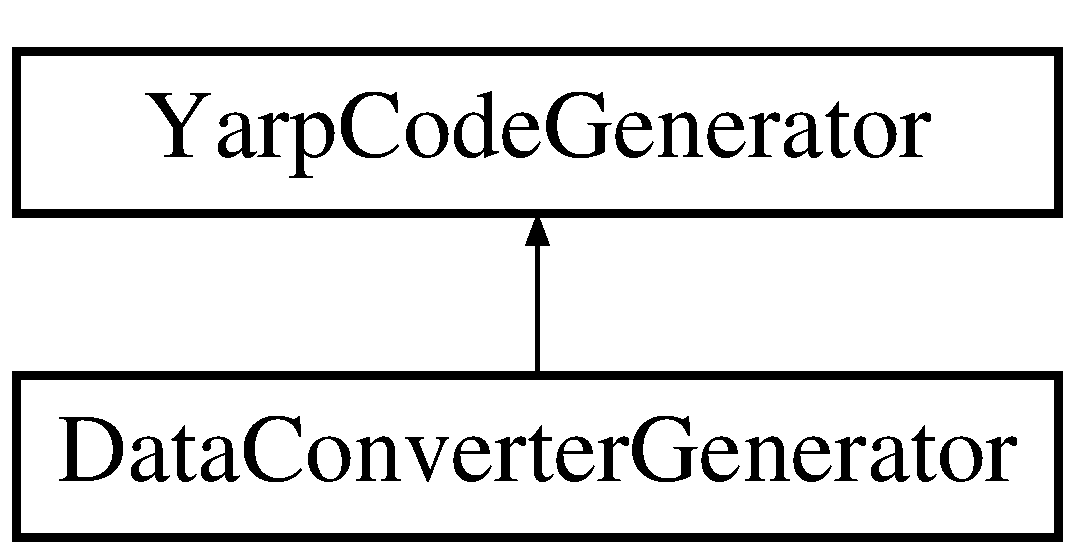
\includegraphics[height=2.000000cm]{classDataConverterGenerator}
\end{center}
\end{figure}
\subsection*{Public Member Functions}
\begin{DoxyCompactItemize}
\item 
\hyperlink{classDataConverterGenerator_a039ab1bff2a8c13f37f994fd4e8b6c57}{Data\-Converter\-Generator} ()
\item 
\hypertarget{classDataConverterGenerator_acdf2a94539b4620df361d752133456d3}{std\-::vector$<$ std\-::string $>$ {\bfseries get\-Function} ()}\label{classDataConverterGenerator_acdf2a94539b4620df361d752133456d3}

\item 
\hypertarget{classDataConverterGenerator_ace67193c92c3b283a147682312e7a7c7}{std\-::vector$<$ bool $>$ {\bfseries get\-Verbose} ()}\label{classDataConverterGenerator_ace67193c92c3b283a147682312e7a7c7}

\item 
\hypertarget{classDataConverterGenerator_a4cfb90e1a29cca7c12e7c93920df4d0d}{void {\bfseries add\-Converter\-Function} (std\-::string function)}\label{classDataConverterGenerator_a4cfb90e1a29cca7c12e7c93920df4d0d}

\item 
\hypertarget{classDataConverterGenerator_a07715c14eac58aaf162f5b7ff36d5ba9}{void {\bfseries add\-Converter\-Verbose} (bool verbose)}\label{classDataConverterGenerator_a07715c14eac58aaf162f5b7ff36d5ba9}

\item 
\hypertarget{classDataConverterGenerator_a1507dd8a542780ffeb277a2bf0a4fbba}{std\-::string {\bfseries get\-Converter\-Function} (int converter\-Index)}\label{classDataConverterGenerator_a1507dd8a542780ffeb277a2bf0a4fbba}

\item 
\hypertarget{classDataConverterGenerator_af74c8edbedcf06eaf33fdccbc6beddac}{bool {\bfseries get\-Converter\-Verbose} (int converter\-Index)}\label{classDataConverterGenerator_af74c8edbedcf06eaf33fdccbc6beddac}

\item 
std\-::string \hyperlink{classDataConverterGenerator_a1c3df6e22d230512a9091184f315b9ef}{generate\-Code} ()
\end{DoxyCompactItemize}
\subsection*{Private Member Functions}
\begin{DoxyCompactItemize}
\item 
std\-::string \hyperlink{classDataConverterGenerator_a64845e3ce285461b22eabb32af5899ff}{function\-To\-String} (int converter\-Index)
\end{DoxyCompactItemize}
\subsection*{Private Attributes}
\begin{DoxyCompactItemize}
\item 
std\-::vector$<$ std\-::string $>$ \hyperlink{classDataConverterGenerator_a44c9695737d8f682c98f7310351dd74e}{function\-\_\-}
\item 
std\-::vector$<$ bool $>$ \hyperlink{classDataConverterGenerator_aad0f91e34facb40b7540ab39a0f974bd}{verbose\-\_\-}
\end{DoxyCompactItemize}


\subsection{Detailed Description}
Header of the class that generates the code of the converter function for the elements of a hub 

Definition at line 8 of file dataconvertergenerator.\-hpp.



\subsection{Constructor \& Destructor Documentation}
\hypertarget{classDataConverterGenerator_a039ab1bff2a8c13f37f994fd4e8b6c57}{\index{Data\-Converter\-Generator@{Data\-Converter\-Generator}!Data\-Converter\-Generator@{Data\-Converter\-Generator}}
\index{Data\-Converter\-Generator@{Data\-Converter\-Generator}!DataConverterGenerator@{Data\-Converter\-Generator}}
\subsubsection[{Data\-Converter\-Generator}]{\setlength{\rightskip}{0pt plus 5cm}Data\-Converter\-Generator\-::\-Data\-Converter\-Generator (
\begin{DoxyParamCaption}
{}
\end{DoxyParamCaption}
)}}\label{classDataConverterGenerator_a039ab1bff2a8c13f37f994fd4e8b6c57}
Constructor

Implementation of the class that generates the code of the converter function for the elements of a hub 

Definition at line 12 of file dataconvertergenerator.\-cpp.



\subsection{Member Function Documentation}
\hypertarget{classDataConverterGenerator_a64845e3ce285461b22eabb32af5899ff}{\index{Data\-Converter\-Generator@{Data\-Converter\-Generator}!function\-To\-String@{function\-To\-String}}
\index{function\-To\-String@{function\-To\-String}!DataConverterGenerator@{Data\-Converter\-Generator}}
\subsubsection[{function\-To\-String}]{\setlength{\rightskip}{0pt plus 5cm}std\-::string Data\-Converter\-Generator\-::function\-To\-String (
\begin{DoxyParamCaption}
\item[{int}]{converter\-Index}
\end{DoxyParamCaption}
)\hspace{0.3cm}{\ttfamily [private]}}}\label{classDataConverterGenerator_a64845e3ce285461b22eabb32af5899ff}
Returns the string containing the code of the converter function. One can add new functions to this method in order to expand the functionality of the converter, but try to document what kind of objects should the mux result have. Example\-: the function deg\-\_\-to\-\_\-rad expects a mutex containing doubles. 
\begin{DoxyParams}{Parameters}
{\em converter\-Index} & identifier in the array of functions of this particular hub \\
\hline
\end{DoxyParams}
\begin{DoxyReturn}{Returns}
std\-::string line(s) of code that performs the data conversion 
\end{DoxyReturn}


Definition at line 65 of file dataconvertergenerator.\-cpp.

\hypertarget{classDataConverterGenerator_a1c3df6e22d230512a9091184f315b9ef}{\index{Data\-Converter\-Generator@{Data\-Converter\-Generator}!generate\-Code@{generate\-Code}}
\index{generate\-Code@{generate\-Code}!DataConverterGenerator@{Data\-Converter\-Generator}}
\subsubsection[{generate\-Code}]{\setlength{\rightskip}{0pt plus 5cm}std\-::string Data\-Converter\-Generator\-::generate\-Code (
\begin{DoxyParamCaption}
{}
\end{DoxyParamCaption}
)\hspace{0.3cm}{\ttfamily [virtual]}}}\label{classDataConverterGenerator_a1c3df6e22d230512a9091184f315b9ef}
Method that implements the code generation \begin{DoxyReturn}{Returns}
String that contains the code 
\end{DoxyReturn}


Implements \hyperlink{classYarpCodeGenerator_ad4247b4dad2a694c3799d5a6968faa41}{Yarp\-Code\-Generator}.



Definition at line 44 of file dataconvertergenerator.\-cpp.



\subsection{Member Data Documentation}
\hypertarget{classDataConverterGenerator_a44c9695737d8f682c98f7310351dd74e}{\index{Data\-Converter\-Generator@{Data\-Converter\-Generator}!function\-\_\-@{function\-\_\-}}
\index{function\-\_\-@{function\-\_\-}!DataConverterGenerator@{Data\-Converter\-Generator}}
\subsubsection[{function\-\_\-}]{\setlength{\rightskip}{0pt plus 5cm}std\-::vector$<$std\-::string$>$ Data\-Converter\-Generator\-::function\-\_\-\hspace{0.3cm}{\ttfamily [private]}}}\label{classDataConverterGenerator_a44c9695737d8f682c98f7310351dd74e}
converter function name 

Definition at line 31 of file dataconvertergenerator.\-hpp.

\hypertarget{classDataConverterGenerator_aad0f91e34facb40b7540ab39a0f974bd}{\index{Data\-Converter\-Generator@{Data\-Converter\-Generator}!verbose\-\_\-@{verbose\-\_\-}}
\index{verbose\-\_\-@{verbose\-\_\-}!DataConverterGenerator@{Data\-Converter\-Generator}}
\subsubsection[{verbose\-\_\-}]{\setlength{\rightskip}{0pt plus 5cm}std\-::vector$<$bool$>$ Data\-Converter\-Generator\-::verbose\-\_\-\hspace{0.3cm}{\ttfamily [private]}}}\label{classDataConverterGenerator_aad0f91e34facb40b7540ab39a0f974bd}
Verbose flag 

Definition at line 32 of file dataconvertergenerator.\-hpp.



The documentation for this class was generated from the following files\-:\begin{DoxyCompactItemize}
\item 
dataconvertergenerator.\-hpp\item 
dataconvertergenerator.\-cpp\end{DoxyCompactItemize}

\hypertarget{classPortMuxGenerator}{\section{Port\-Mux\-Generator Class Reference}
\label{classPortMuxGenerator}\index{Port\-Mux\-Generator@{Port\-Mux\-Generator}}
}


{\ttfamily \#include $<$portmuxgenerator.\-hpp$>$}

Inheritance diagram for Port\-Mux\-Generator\-:\begin{figure}[H]
\begin{center}
\leavevmode
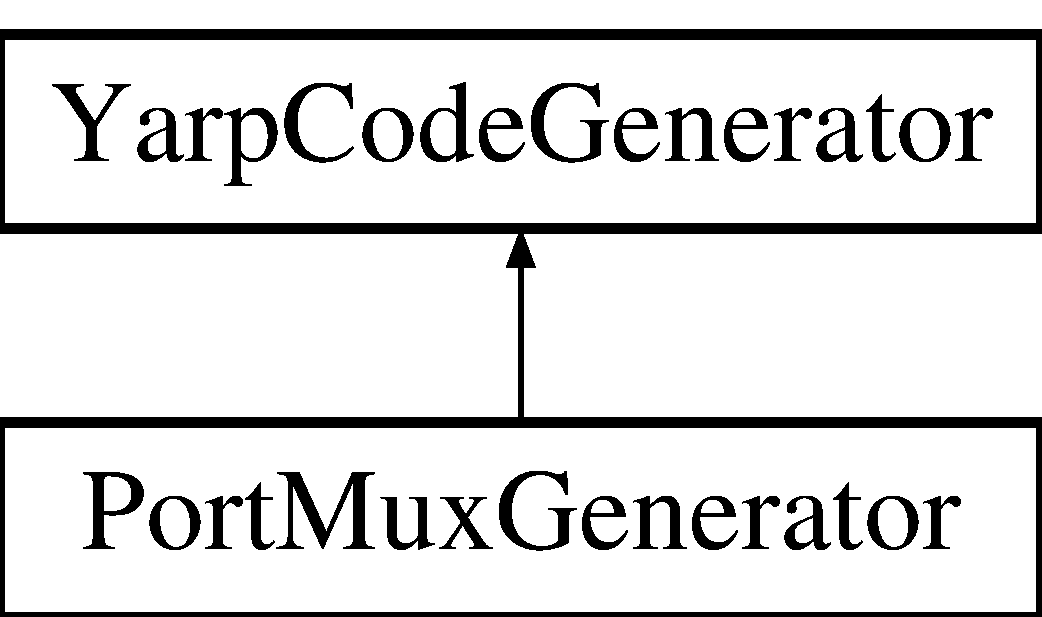
\includegraphics[height=2.000000cm]{classPortMuxGenerator}
\end{center}
\end{figure}
\subsection*{Public Member Functions}
\begin{DoxyCompactItemize}
\item 
\hyperlink{classPortMuxGenerator_a88f5396d5f7564ad04d74d0184ab6e83}{Port\-Mux\-Generator} (int num\-Muxes, std\-::string output\-Name, bool to\-Ros, std\-::string \&output\-\_\-port\-\_\-name\-\_\-, std\-::string \&ros\-\_\-message\-\_\-name, bool from\-Ros)
\item 
\hyperlink{classPortMuxGenerator_afb0616d1f35b218b08f9482a30322d32}{$\sim$\-Port\-Mux\-Generator} ()
\item 
\hypertarget{classPortMuxGenerator_ade9b337018f7e2794efb4ec69f790af1}{int {\bfseries get\-Num\-Muxes} ()}\label{classPortMuxGenerator_ade9b337018f7e2794efb4ec69f790af1}

\item 
\hypertarget{classPortMuxGenerator_aa92143f0290965c23e1f727ad0aea5e1}{std\-::string {\bfseries get\-Output\-Name} ()}\label{classPortMuxGenerator_aa92143f0290965c23e1f727ad0aea5e1}

\item 
\hypertarget{classPortMuxGenerator_a6dc487c1749d7af1e22a0f738dab9705}{std\-::string {\bfseries get\-Ros\-Message\-Name} ()}\label{classPortMuxGenerator_a6dc487c1749d7af1e22a0f738dab9705}

\item 
\hypertarget{classPortMuxGenerator_a1ba37b470422d906d9aa287524548fd5}{bool {\bfseries get\-To\-Ros} ()}\label{classPortMuxGenerator_a1ba37b470422d906d9aa287524548fd5}

\item 
\hypertarget{classPortMuxGenerator_a150ec5e8d2b45896a22c37e967a5bdc9}{bool {\bfseries get\-From\-Ros} ()}\label{classPortMuxGenerator_a150ec5e8d2b45896a22c37e967a5bdc9}

\item 
\hypertarget{classPortMuxGenerator_a432c713e00d15a0f330c2811887ca8ff}{std\-::vector$<$ int $>$ {\bfseries get\-Num\-Ports} ()}\label{classPortMuxGenerator_a432c713e00d15a0f330c2811887ca8ff}

\item 
\hypertarget{classPortMuxGenerator_aa1c438d531d3e3418f135d6c7041279d}{std\-::vector$<$ std\-::string $>$ {\bfseries get\-Ports} ()}\label{classPortMuxGenerator_aa1c438d531d3e3418f135d6c7041279d}

\item 
\hypertarget{classPortMuxGenerator_a956196e2654ec5e7958a9cb98bde7a9b}{void {\bfseries add\-Mux\-Num\-Ports} (int num\-Ports)}\label{classPortMuxGenerator_a956196e2654ec5e7958a9cb98bde7a9b}

\item 
void \hyperlink{classPortMuxGenerator_ac1899aadf7ded799355b58efe03f4ce2}{add\-Mux\-Ports} (std\-::string ports)
\item 
int \hyperlink{classPortMuxGenerator_a8abf12f10f752f2919e34fab9855770a}{get\-Mux\-Num\-Ports} (int mux\-Index)
\item 
std\-::string \hyperlink{classPortMuxGenerator_a17cd5018bbe6c9bc5e2ceca94375a1af}{get\-Mux\-Ports} (int mux\-Index)
\item 
std\-::string \hyperlink{classPortMuxGenerator_a0f740d798c16c0dee5de7b6fbace3c53}{generate\-Code} ()
\end{DoxyCompactItemize}
\subsection*{Private Member Functions}
\begin{DoxyCompactItemize}
\item 
std\-::string \hyperlink{classPortMuxGenerator_a3fdfcabf997e4f8d89a42776c0a1c2bc}{extract\-Port\-From\-String} (int mux\-Index, int port\-Index)
\end{DoxyCompactItemize}
\subsection*{Private Attributes}
\begin{DoxyCompactItemize}
\item 
int \hyperlink{classPortMuxGenerator_a48cec4ed3c40d0fb987a85dbcb2f02ac}{num\-Muxes\-\_\-}
\item 
std\-::string \hyperlink{classPortMuxGenerator_a6c459791ee05d68f48e087b4d3cedc68}{output\-Name\-\_\-}
\item 
std\-::string \hyperlink{classPortMuxGenerator_a78f4039de899ad9af05bb7d72cf310b7}{ros\-Message\-Name\-\_\-}
\item 
bool \hyperlink{classPortMuxGenerator_ada967c8c94e76a6b73598e77b039086b}{to\-Ros\-\_\-}
\item 
bool \hyperlink{classPortMuxGenerator_ab3876f874fe7230a5585d203cda2ff3b}{from\-Ros\-\_\-}
\item 
std\-::vector$<$ int $>$ \hyperlink{classPortMuxGenerator_addec6f43a703f42fe99a3fc8f877dd1d}{num\-Ports\-\_\-}
\item 
std\-::vector$<$ std\-::string $>$ \hyperlink{classPortMuxGenerator_a05ea2374bbae5e1c1bb069a793a3685e}{ports\-\_\-}
\item 
std\-::string \hyperlink{classPortMuxGenerator_a8a342f9a1ea4fea5be14d05f0ff4b251}{output\-\_\-port\-\_\-name}
\end{DoxyCompactItemize}


\subsection{Detailed Description}
Class that generates the code for connecting and reading the values from the input Y\-A\-R\-P ports/\-R\-O\-S topics 

Definition at line 8 of file portmuxgenerator.\-hpp.



\subsection{Constructor \& Destructor Documentation}
\hypertarget{classPortMuxGenerator_a88f5396d5f7564ad04d74d0184ab6e83}{\index{Port\-Mux\-Generator@{Port\-Mux\-Generator}!Port\-Mux\-Generator@{Port\-Mux\-Generator}}
\index{Port\-Mux\-Generator@{Port\-Mux\-Generator}!PortMuxGenerator@{Port\-Mux\-Generator}}
\subsubsection[{Port\-Mux\-Generator}]{\setlength{\rightskip}{0pt plus 5cm}Port\-Mux\-Generator\-::\-Port\-Mux\-Generator (
\begin{DoxyParamCaption}
\item[{int}]{num\-Muxes, }
\item[{std\-::string}]{output\-Name, }
\item[{bool}]{to\-Ros, }
\item[{std\-::string \&}]{output\-\_\-port\-\_\-name\-\_\-, }
\item[{std\-::string \&}]{ros\-\_\-message\-\_\-name, }
\item[{bool}]{from\-Ros}
\end{DoxyParamCaption}
)}}\label{classPortMuxGenerator_a88f5396d5f7564ad04d74d0184ab6e83}
Constructor 
\begin{DoxyParams}{Parameters}
{\em num\-Muxes} & Number of hubs \\
\hline
{\em output\-Name} & Y\-A\-R\-P port/\-R\-O\-S topic where the output will be send \\
\hline
{\em to\-Ros} & Boolean flag to know the type of output (R\-O\-S message or Y\-A\-R\-P Bottle) \\
\hline
{\em output\-\_\-port\-\_\-name\-\_\-} & Folder name where the code will be copied \\
\hline
{\em ros\-\_\-message\-\_\-name} & When writing to a R\-O\-S topic, this is the R\-O\-S message name \\
\hline
{\em from\-Ros} & Boolean flag to know the type of inputs (R\-O\-S message or Y\-A\-R\-P Bottle) \\
\hline
\end{DoxyParams}


Definition at line 9 of file portmuxgenerator.\-cpp.

\hypertarget{classPortMuxGenerator_afb0616d1f35b218b08f9482a30322d32}{\index{Port\-Mux\-Generator@{Port\-Mux\-Generator}!$\sim$\-Port\-Mux\-Generator@{$\sim$\-Port\-Mux\-Generator}}
\index{$\sim$\-Port\-Mux\-Generator@{$\sim$\-Port\-Mux\-Generator}!PortMuxGenerator@{Port\-Mux\-Generator}}
\subsubsection[{$\sim$\-Port\-Mux\-Generator}]{\setlength{\rightskip}{0pt plus 5cm}Port\-Mux\-Generator\-::$\sim$\-Port\-Mux\-Generator (
\begin{DoxyParamCaption}
{}
\end{DoxyParamCaption}
)}}\label{classPortMuxGenerator_afb0616d1f35b218b08f9482a30322d32}
Destructor 

Definition at line 19 of file portmuxgenerator.\-cpp.



\subsection{Member Function Documentation}
\hypertarget{classPortMuxGenerator_ac1899aadf7ded799355b58efe03f4ce2}{\index{Port\-Mux\-Generator@{Port\-Mux\-Generator}!add\-Mux\-Ports@{add\-Mux\-Ports}}
\index{add\-Mux\-Ports@{add\-Mux\-Ports}!PortMuxGenerator@{Port\-Mux\-Generator}}
\subsubsection[{add\-Mux\-Ports}]{\setlength{\rightskip}{0pt plus 5cm}void Port\-Mux\-Generator\-::add\-Mux\-Ports (
\begin{DoxyParamCaption}
\item[{std\-::string}]{ports}
\end{DoxyParamCaption}
)}}\label{classPortMuxGenerator_ac1899aadf7ded799355b58efe03f4ce2}
Adds the ports/topics string of a hub 
\begin{DoxyParams}{Parameters}
{\em ports} & String with comma separated ports/topics \\
\hline
\end{DoxyParams}


Definition at line 52 of file portmuxgenerator.\-cpp.

\hypertarget{classPortMuxGenerator_a3fdfcabf997e4f8d89a42776c0a1c2bc}{\index{Port\-Mux\-Generator@{Port\-Mux\-Generator}!extract\-Port\-From\-String@{extract\-Port\-From\-String}}
\index{extract\-Port\-From\-String@{extract\-Port\-From\-String}!PortMuxGenerator@{Port\-Mux\-Generator}}
\subsubsection[{extract\-Port\-From\-String}]{\setlength{\rightskip}{0pt plus 5cm}std\-::string Port\-Mux\-Generator\-::extract\-Port\-From\-String (
\begin{DoxyParamCaption}
\item[{int}]{mux\-Index, }
\item[{int}]{port\-Index}
\end{DoxyParamCaption}
)\hspace{0.3cm}{\ttfamily [private]}}}\label{classPortMuxGenerator_a3fdfcabf997e4f8d89a42776c0a1c2bc}
Retrieve port/topic name from wrap of ports names. Requires names separated by commas and no spaces between them. 
\begin{DoxyParams}{Parameters}
{\em mux\-Index} & Hub's index in the vector of Hubs \\
\hline
{\em port\-Index} & Port's index in the ports string \\
\hline
\end{DoxyParams}


Definition at line 182 of file portmuxgenerator.\-cpp.

\hypertarget{classPortMuxGenerator_a0f740d798c16c0dee5de7b6fbace3c53}{\index{Port\-Mux\-Generator@{Port\-Mux\-Generator}!generate\-Code@{generate\-Code}}
\index{generate\-Code@{generate\-Code}!PortMuxGenerator@{Port\-Mux\-Generator}}
\subsubsection[{generate\-Code}]{\setlength{\rightskip}{0pt plus 5cm}std\-::string Port\-Mux\-Generator\-::generate\-Code (
\begin{DoxyParamCaption}
{}
\end{DoxyParamCaption}
)\hspace{0.3cm}{\ttfamily [virtual]}}}\label{classPortMuxGenerator_a0f740d798c16c0dee5de7b6fbace3c53}
Generates the code that connects to all the Y\-A\-R\-P ports/\-R\-O\-S topics \begin{DoxyReturn}{Returns}
String that contains the code for Y\-A\-R\-P port creation, and connection to the input Y\-A\-R\-P ports/\-R\-O\-S topics 
\end{DoxyReturn}


Implements \hyperlink{classYarpCodeGenerator_ad4247b4dad2a694c3799d5a6968faa41}{Yarp\-Code\-Generator}.



Definition at line 64 of file portmuxgenerator.\-cpp.

\hypertarget{classPortMuxGenerator_a8abf12f10f752f2919e34fab9855770a}{\index{Port\-Mux\-Generator@{Port\-Mux\-Generator}!get\-Mux\-Num\-Ports@{get\-Mux\-Num\-Ports}}
\index{get\-Mux\-Num\-Ports@{get\-Mux\-Num\-Ports}!PortMuxGenerator@{Port\-Mux\-Generator}}
\subsubsection[{get\-Mux\-Num\-Ports}]{\setlength{\rightskip}{0pt plus 5cm}int Port\-Mux\-Generator\-::get\-Mux\-Num\-Ports (
\begin{DoxyParamCaption}
\item[{int}]{mux\-Index}
\end{DoxyParamCaption}
)}}\label{classPortMuxGenerator_a8abf12f10f752f2919e34fab9855770a}
Returns the number of ports read by the hub at mux\-Index in the hub vector 
\begin{DoxyParams}{Parameters}
{\em mux\-Index} & Hub index in the Hub vector \\
\hline
\end{DoxyParams}
\begin{DoxyReturn}{Returns}
int Number of ports/topics read by the hub 
\end{DoxyReturn}


Definition at line 56 of file portmuxgenerator.\-cpp.

\hypertarget{classPortMuxGenerator_a17cd5018bbe6c9bc5e2ceca94375a1af}{\index{Port\-Mux\-Generator@{Port\-Mux\-Generator}!get\-Mux\-Ports@{get\-Mux\-Ports}}
\index{get\-Mux\-Ports@{get\-Mux\-Ports}!PortMuxGenerator@{Port\-Mux\-Generator}}
\subsubsection[{get\-Mux\-Ports}]{\setlength{\rightskip}{0pt plus 5cm}std\-::string Port\-Mux\-Generator\-::get\-Mux\-Ports (
\begin{DoxyParamCaption}
\item[{int}]{mux\-Index}
\end{DoxyParamCaption}
)}}\label{classPortMuxGenerator_a17cd5018bbe6c9bc5e2ceca94375a1af}
Returns the string that contains all the Y\-A\-R\-P ports/\-R\-O\-S topics for the hub mux\-Index 
\begin{DoxyParams}{Parameters}
{\em mux\-Index} & Hub index in the Hub vector \\
\hline
\end{DoxyParams}
\begin{DoxyReturn}{Returns}
String that contains the Y\-A\-R\-P ports/\-R\-O\-S topics separated by commas 
\end{DoxyReturn}


Definition at line 60 of file portmuxgenerator.\-cpp.



\subsection{Member Data Documentation}
\hypertarget{classPortMuxGenerator_ab3876f874fe7230a5585d203cda2ff3b}{\index{Port\-Mux\-Generator@{Port\-Mux\-Generator}!from\-Ros\-\_\-@{from\-Ros\-\_\-}}
\index{from\-Ros\-\_\-@{from\-Ros\-\_\-}!PortMuxGenerator@{Port\-Mux\-Generator}}
\subsubsection[{from\-Ros\-\_\-}]{\setlength{\rightskip}{0pt plus 5cm}bool Port\-Mux\-Generator\-::from\-Ros\-\_\-\hspace{0.3cm}{\ttfamily [private]}}}\label{classPortMuxGenerator_ab3876f874fe7230a5585d203cda2ff3b}
Boolean flag to know the type of inputs (R\-O\-S message or Y\-A\-R\-P Bottle) 

Definition at line 71 of file portmuxgenerator.\-hpp.

\hypertarget{classPortMuxGenerator_a48cec4ed3c40d0fb987a85dbcb2f02ac}{\index{Port\-Mux\-Generator@{Port\-Mux\-Generator}!num\-Muxes\-\_\-@{num\-Muxes\-\_\-}}
\index{num\-Muxes\-\_\-@{num\-Muxes\-\_\-}!PortMuxGenerator@{Port\-Mux\-Generator}}
\subsubsection[{num\-Muxes\-\_\-}]{\setlength{\rightskip}{0pt plus 5cm}int Port\-Mux\-Generator\-::num\-Muxes\-\_\-\hspace{0.3cm}{\ttfamily [private]}}}\label{classPortMuxGenerator_a48cec4ed3c40d0fb987a85dbcb2f02ac}
Number of hubs 

Definition at line 67 of file portmuxgenerator.\-hpp.

\hypertarget{classPortMuxGenerator_addec6f43a703f42fe99a3fc8f877dd1d}{\index{Port\-Mux\-Generator@{Port\-Mux\-Generator}!num\-Ports\-\_\-@{num\-Ports\-\_\-}}
\index{num\-Ports\-\_\-@{num\-Ports\-\_\-}!PortMuxGenerator@{Port\-Mux\-Generator}}
\subsubsection[{num\-Ports\-\_\-}]{\setlength{\rightskip}{0pt plus 5cm}std\-::vector$<$int$>$ Port\-Mux\-Generator\-::num\-Ports\-\_\-\hspace{0.3cm}{\ttfamily [private]}}}\label{classPortMuxGenerator_addec6f43a703f42fe99a3fc8f877dd1d}
Vector that contains the number of ports for all the hubs 

Definition at line 72 of file portmuxgenerator.\-hpp.

\hypertarget{classPortMuxGenerator_a8a342f9a1ea4fea5be14d05f0ff4b251}{\index{Port\-Mux\-Generator@{Port\-Mux\-Generator}!output\-\_\-port\-\_\-name@{output\-\_\-port\-\_\-name}}
\index{output\-\_\-port\-\_\-name@{output\-\_\-port\-\_\-name}!PortMuxGenerator@{Port\-Mux\-Generator}}
\subsubsection[{output\-\_\-port\-\_\-name}]{\setlength{\rightskip}{0pt plus 5cm}std\-::string Port\-Mux\-Generator\-::output\-\_\-port\-\_\-name\hspace{0.3cm}{\ttfamily [private]}}}\label{classPortMuxGenerator_a8a342f9a1ea4fea5be14d05f0ff4b251}
Folder name where the code will be copied 

Definition at line 74 of file portmuxgenerator.\-hpp.

\hypertarget{classPortMuxGenerator_a6c459791ee05d68f48e087b4d3cedc68}{\index{Port\-Mux\-Generator@{Port\-Mux\-Generator}!output\-Name\-\_\-@{output\-Name\-\_\-}}
\index{output\-Name\-\_\-@{output\-Name\-\_\-}!PortMuxGenerator@{Port\-Mux\-Generator}}
\subsubsection[{output\-Name\-\_\-}]{\setlength{\rightskip}{0pt plus 5cm}std\-::string Port\-Mux\-Generator\-::output\-Name\-\_\-\hspace{0.3cm}{\ttfamily [private]}}}\label{classPortMuxGenerator_a6c459791ee05d68f48e087b4d3cedc68}
Y\-A\-R\-P port/\-R\-O\-S topic where the output will be send 

Definition at line 68 of file portmuxgenerator.\-hpp.

\hypertarget{classPortMuxGenerator_a05ea2374bbae5e1c1bb069a793a3685e}{\index{Port\-Mux\-Generator@{Port\-Mux\-Generator}!ports\-\_\-@{ports\-\_\-}}
\index{ports\-\_\-@{ports\-\_\-}!PortMuxGenerator@{Port\-Mux\-Generator}}
\subsubsection[{ports\-\_\-}]{\setlength{\rightskip}{0pt plus 5cm}std\-::vector$<$std\-::string$>$ Port\-Mux\-Generator\-::ports\-\_\-\hspace{0.3cm}{\ttfamily [private]}}}\label{classPortMuxGenerator_a05ea2374bbae5e1c1bb069a793a3685e}
Vector that contains the inputs (ports/topics) for all the hubs 

Definition at line 73 of file portmuxgenerator.\-hpp.

\hypertarget{classPortMuxGenerator_a78f4039de899ad9af05bb7d72cf310b7}{\index{Port\-Mux\-Generator@{Port\-Mux\-Generator}!ros\-Message\-Name\-\_\-@{ros\-Message\-Name\-\_\-}}
\index{ros\-Message\-Name\-\_\-@{ros\-Message\-Name\-\_\-}!PortMuxGenerator@{Port\-Mux\-Generator}}
\subsubsection[{ros\-Message\-Name\-\_\-}]{\setlength{\rightskip}{0pt plus 5cm}std\-::string Port\-Mux\-Generator\-::ros\-Message\-Name\-\_\-\hspace{0.3cm}{\ttfamily [private]}}}\label{classPortMuxGenerator_a78f4039de899ad9af05bb7d72cf310b7}
When writing to a R\-O\-S topic, this is the R\-O\-S message name 

Definition at line 69 of file portmuxgenerator.\-hpp.

\hypertarget{classPortMuxGenerator_ada967c8c94e76a6b73598e77b039086b}{\index{Port\-Mux\-Generator@{Port\-Mux\-Generator}!to\-Ros\-\_\-@{to\-Ros\-\_\-}}
\index{to\-Ros\-\_\-@{to\-Ros\-\_\-}!PortMuxGenerator@{Port\-Mux\-Generator}}
\subsubsection[{to\-Ros\-\_\-}]{\setlength{\rightskip}{0pt plus 5cm}bool Port\-Mux\-Generator\-::to\-Ros\-\_\-\hspace{0.3cm}{\ttfamily [private]}}}\label{classPortMuxGenerator_ada967c8c94e76a6b73598e77b039086b}
Boolean flag to know the type of output (R\-O\-S message or Y\-A\-R\-P Bottle) 

Definition at line 70 of file portmuxgenerator.\-hpp.



The documentation for this class was generated from the following files\-:\begin{DoxyCompactItemize}
\item 
portmuxgenerator.\-hpp\item 
portmuxgenerator.\-cpp\end{DoxyCompactItemize}

\hypertarget{classYarpCodeGenerator}{\section{Yarp\-Code\-Generator Class Reference}
\label{classYarpCodeGenerator}\index{Yarp\-Code\-Generator@{Yarp\-Code\-Generator}}
}


{\ttfamily \#include $<$yarpcodegenerator.\-hpp$>$}

Inheritance diagram for Yarp\-Code\-Generator\-:\begin{figure}[H]
\begin{center}
\leavevmode
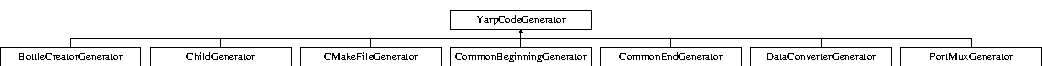
\includegraphics[height=0.883978cm]{classYarpCodeGenerator}
\end{center}
\end{figure}
\subsection*{Public Member Functions}
\begin{DoxyCompactItemize}
\item 
virtual std\-::string \hyperlink{classYarpCodeGenerator_ad4247b4dad2a694c3799d5a6968faa41}{generate\-Code} ()=0
\end{DoxyCompactItemize}


\subsection{Detailed Description}
Interface that represents which will be implemented by all the code generating classes 

Definition at line 6 of file yarpcodegenerator.\-hpp.



\subsection{Member Function Documentation}
\hypertarget{classYarpCodeGenerator_ad4247b4dad2a694c3799d5a6968faa41}{\index{Yarp\-Code\-Generator@{Yarp\-Code\-Generator}!generate\-Code@{generate\-Code}}
\index{generate\-Code@{generate\-Code}!YarpCodeGenerator@{Yarp\-Code\-Generator}}
\subsubsection[{generate\-Code}]{\setlength{\rightskip}{0pt plus 5cm}virtual std\-::string Yarp\-Code\-Generator\-::generate\-Code (
\begin{DoxyParamCaption}
{}
\end{DoxyParamCaption}
)\hspace{0.3cm}{\ttfamily [pure virtual]}}}\label{classYarpCodeGenerator_ad4247b4dad2a694c3799d5a6968faa41}
Method that implements the code generation \begin{DoxyReturn}{Returns}
String that contains the code 
\end{DoxyReturn}


Implemented in \hyperlink{classPortMuxGenerator_a0f740d798c16c0dee5de7b6fbace3c53}{Port\-Mux\-Generator}, \hyperlink{classBottleCreatorGenerator_a71d28a76d750bcfa2de6f62f8b9b5a62}{Bottle\-Creator\-Generator}, \hyperlink{classChildGenerator_a2dd3b214edfe346d16c8c2cdc708cc52}{Child\-Generator}, \hyperlink{classDataConverterGenerator_a1c3df6e22d230512a9091184f315b9ef}{Data\-Converter\-Generator}, \hyperlink{classCMakeFileGenerator_a5505ce5e4f9397e616f521e70f56f9d7}{C\-Make\-File\-Generator}, \hyperlink{classCommonBeginningGenerator_a34d951b06ae3658659b2c76e3bbb1413}{Common\-Beginning\-Generator}, and \hyperlink{classCommonEndGenerator_a08904bf31bed7b708155b354ab33e272}{Common\-End\-Generator}.



The documentation for this class was generated from the following files\-:\begin{DoxyCompactItemize}
\item 
yarpcodegenerator.\-hpp\item 
yarpcodegenerator.\-cpp\end{DoxyCompactItemize}

\chapter{File Documentation}
\hypertarget{main_8cpp}{\section{main.\-cpp File Reference}
\label{main_8cpp}\index{main.\-cpp@{main.\-cpp}}
}
{\ttfamily \#include $<$iostream$>$}\\*
{\ttfamily \#include $<$fstream$>$}\\*
{\ttfamily \#include \char`\"{}commonbeginninggenerator.\-hpp\char`\"{}}\\*
{\ttfamily \#include \char`\"{}portmuxgenerator.\-hpp\char`\"{}}\\*
{\ttfamily \#include \char`\"{}dataconvertergenerator.\-hpp\char`\"{}}\\*
{\ttfamily \#include \char`\"{}bottlecreatorgenerator.\-hpp\char`\"{}}\\*
{\ttfamily \#include \char`\"{}cmakefilegenerator.\-hpp\char`\"{}}\\*
{\ttfamily \#include \char`\"{}commonendgenerator.\-hpp\char`\"{}}\\*
{\ttfamily \#include $<$boost/property\-\_\-tree/ptree.\-hpp$>$}\\*
{\ttfamily \#include $<$boost/property\-\_\-tree/ini\-\_\-parser.\-hpp$>$}\\*
{\ttfamily \#include $<$boost/lexical\-\_\-cast.\-hpp$>$}\\*
{\ttfamily \#include $<$boost/filesystem.\-hpp$>$}\\*
\subsection*{Functions}
\begin{DoxyCompactItemize}
\item 
void \hyperlink{main_8cpp_aa068cf952519028e73fc42cadc625ede}{handle\-Message\-Child} (\hyperlink{classChildGenerator}{Child\-Generator} \&child\-Gen, boost\-::property\-\_\-tree\-::ptree \&pt, std\-::string message\-Name, bool to\-Ros)
\item 
void \hyperlink{main_8cpp_aa668161c343a125980df234982c54f90}{handle\-Message\-Fields} (\hyperlink{classBottleCreatorGenerator}{Bottle\-Creator\-Generator} \&bottle\-Creator\-Gen, boost\-::property\-\_\-tree\-::ptree \&pt, bool to\-Ros)
\item 
void \hyperlink{main_8cpp_ac1b66fe77173de9e5e8542b2823d6071}{info} ()
\item 
\hypertarget{main_8cpp_a0ddf1224851353fc92bfbff6f499fa97}{int {\bfseries main} (int argc, char $\ast$argv\mbox{[}$\,$\mbox{]})}\label{main_8cpp_a0ddf1224851353fc92bfbff6f499fa97}

\end{DoxyCompactItemize}


\subsection{Function Documentation}
\hypertarget{main_8cpp_aa068cf952519028e73fc42cadc625ede}{\index{main.\-cpp@{main.\-cpp}!handle\-Message\-Child@{handle\-Message\-Child}}
\index{handle\-Message\-Child@{handle\-Message\-Child}!main.cpp@{main.\-cpp}}
\subsubsection[{handle\-Message\-Child}]{\setlength{\rightskip}{0pt plus 5cm}void handle\-Message\-Child (
\begin{DoxyParamCaption}
\item[{{\bf Child\-Generator} \&}]{child\-Gen, }
\item[{boost\-::property\-\_\-tree\-::ptree \&}]{pt, }
\item[{std\-::string}]{message\-Name, }
\item[{bool}]{to\-Ros}
\end{DoxyParamCaption}
)}}\label{main_8cpp_aa068cf952519028e73fc42cadc625ede}
Initialize the child objects (tree leaves) from the configuration file 
\begin{DoxyParams}{Parameters}
{\em child\-Gen} & \hyperlink{classChildGenerator}{Child\-Generator} object reference to be initialized from the configuration file \\
\hline
{\em pt} & boost\-::property\-\_\-tree that contains the configuration file data \\
\hline
{\em message\-Name} & R\-O\-S message name, used when the boolean to\-Ros is true \\
\hline
{\em to\-Ros} & Boolean flag to know the type of output \\
\hline
\end{DoxyParams}


Definition at line 37 of file main.\-cpp.

\hypertarget{main_8cpp_aa668161c343a125980df234982c54f90}{\index{main.\-cpp@{main.\-cpp}!handle\-Message\-Fields@{handle\-Message\-Fields}}
\index{handle\-Message\-Fields@{handle\-Message\-Fields}!main.cpp@{main.\-cpp}}
\subsubsection[{handle\-Message\-Fields}]{\setlength{\rightskip}{0pt plus 5cm}void handle\-Message\-Fields (
\begin{DoxyParamCaption}
\item[{{\bf Bottle\-Creator\-Generator} \&}]{bottle\-Creator\-Gen, }
\item[{boost\-::property\-\_\-tree\-::ptree \&}]{pt, }
\item[{bool}]{to\-Ros}
\end{DoxyParamCaption}
)}}\label{main_8cpp_aa668161c343a125980df234982c54f90}
Initialize the objects at the top of the hierarchy (members of the root) from the configuration file 
\begin{DoxyParams}{Parameters}
{\em bottle\-Creator\-Gen} & \hyperlink{classBottleCreatorGenerator}{Bottle\-Creator\-Generator} object reference to be initialized from the configuration file \\
\hline
{\em pt} & boost\-::property\-\_\-tree that contains the configuration file data \\
\hline
{\em to\-Ros} & Boolean flag to know the type of output \\
\hline
\end{DoxyParams}


Definition at line 77 of file main.\-cpp.

\hypertarget{main_8cpp_ac1b66fe77173de9e5e8542b2823d6071}{\index{main.\-cpp@{main.\-cpp}!info@{info}}
\index{info@{info}!main.cpp@{main.\-cpp}}
\subsubsection[{info}]{\setlength{\rightskip}{0pt plus 5cm}void info (
\begin{DoxyParamCaption}
{}
\end{DoxyParamCaption}
)}}\label{main_8cpp_ac1b66fe77173de9e5e8542b2823d6071}
Function that prints out the help 

Definition at line 114 of file main.\-cpp.


%--- End generated contents ---

% Index
\newpage
\phantomsection
\addcontentsline{toc}{chapter}{Index}
\printindex

\end{document}
